\chapter{Data Acquisition}
\label{ch:sp-daq}

%%% todo

\fixme{\textbf{Authors:} 

  See \url{https://wiki.dunescience.org/wiki/Technical_Design_Report}
  for general guidance. 

  While this chapter is still in outline, \textbf{check that it hits all
  the required points} some of which are:

  We are to describe a \textbf{baseline} or \textbf{process to
  decide a baseline}.

  \textbf{BE SUCCINCT} $TDR \approx IDR + 10\%$, goal is 50 pages for
  this chapter. 

  You are encouraged to produce \textbf{tech notes} with any
  supporting verbosity which may be referenced.

  State requirements and demonstrate how they are met, use
  standardized requirements table.

  Emphasize safety and professionalism (projectisms: cost, schedule,
  risks, interfaces).}

\metainfo{Some sections of this chapter must be written generically
  and without any reference to module-specific terms. They are marked
  with an orange ``fixme'' box. 
  Yellow info boxes like this one provide guidance for the content. 
  This guidance is not comprehensive so authors may provide additional
  information but retaining \textbf{conciseness} and \textbf{not
    repeating} info in other section is required.}
 
\section{Introduction}
\label{sec:fd-daq:introduction}
% \fixme{module-generic}

% \metainfo{A brief introduction to this chapter describing what will be
%   described.  This is \textbf{not} an overview of the \dword{daq} itself.
%   Keep it brief. Do \textbf{not} write a conceptual overview here,
%   that is below, reference it. 
%   Do \textbf{not} use module-specific language but \textbf{do}
%   describe how commonalities are described in text shared by both
%   SP/DP volumes and specialized sections appear only in their
%   respective volume. 
%   \textbf{Do} describe the lexicographical convention used to demark
%   shared sections (this needs coordination with other chapters in the
%   same boat).}
The \dword{fd} \dword{daq} system provides
timing and synchronization for all \dwords{detmodule} and
subdetectors; receives, synchronizes, compresses, and buffers streaming
data from the subdetectors; extracts information from the data at a
local level to subsequently make local, module, and cross-module data
selection decisions; builds  events %``events''
 from selected space-time volumes 
and relays them to permanent storage; and carries out local data
reduction and filtering of the data as needed.


This chapter provides a description for the design of the \dword{dune}
\dword{fd} \dword{daq} system developed by the \dword{dune} \dword{fd}
\dword{daq} consortium. 
This consortium brings together resources and expertise from CERN,
Columbia, France, Japan, Netherlands the UK, and the USA. 
Its members bring considerable experience from ICARUS, MicroBooNE, and
DUNE prototype LArTPCs, as well as from ATLAS at the LHC and other major
HEP experiments across the world.

The system is designed %so that it 
to service all \dword{fd}
\dwords{detmodule}, and therefore most aspects of the design are
identical across them. % different \dwords{detmodule}. 
%The descriptions for those parts of the system are reproduced verbatim in some sections of this chapter as found in the TDR volume for each \dword{detmodule}.
%A small part 
However, some aspects of the \dword{daq} design must be tailored to meet
module-specific requirements. 
%Those portions of the design 
These aspects are documented in sections of this chapter %which are 
unique to the \dword{detmodule} covered in this TDR volume;  
these sections are %identified 
identifiable by their use of module-specific terms.

The chapter begins with %requirements 
specifications for \dword{daq} 
and interfaces between it and other \dword{dune} systems. 
Subsequently, Section~\ref{sec:fd-daq:protodune} compares the
\dword{protodune} experiment with \dword{dune} in order to highlight
important information already provided by \dword{protodune}, and
future understanding expected by further exploitation of it, as well as what must be understood by other means. 
Section~\ref{sec:fd-daq:design} comprises the bulk of this chapter and
describes the design of the \dword{fd} \dword{daq}. 
Finally, the chapter finishes with details on management of the
\dword{daq} project describing the completion of the design,
production, and installation of the system, as well as cost, schedule and
safety considerations.



\section{Design Overview}
%\section{Requirements}
\label{sec:fd-daq:requirements}
\fixme{module-generic}

The %\dword{dune} \dword{fd} 
\dword{daq} system must meet the
\dword{dune} %top-level 
\dword{fd}-level as well as \dword{daq}-level
requirements. The \dword{fd}-level  requirements that explicitly pertain to
the \dword{daq} are listed below. %The \dword{daq}-level  specifications are 
%listed in Tables~\ref{tab:spec:min-drift-field}~--~\ref{tab:spec:dead-channels}. 
The system is
designed to meet these requirements and does so by following key
specifications provided in Table~\ref{tab:specs:SP-DAQ} and described in Section~\ref{sec:fd-daq:specifications}. 


DUNE has three main physics drivers: neutrino \dword{cpv} %CP violation 
and related
long baseline oscillation studies using the high-intensity beam provided
by \fnal, off-beam measurements of atmospheric neutrinos and searches
for rare processes such decays allowed through baryon number violation,
and detection of \dfirst{snb} occurring within our galaxy.
The \dword{dune} \dword{fd} modules in the current design implement two
detection technologies: \dfirst{tpc} and \dfirst{pds}.

The two technologies access the physics %each 
with very different readout
time scales.
Charge measurement by the \dword{tpc} of an ionizing event requires a
nominal recording of data over a time window of \SIrange{5}{10}{\milli\second}
%in order 
to collect information from the full detector volume. 
This time scale is determined by the ionization electron drift speed in
\lar and the detector dimension along the drift direction.
The \dword{pds} measures argon scintillation light emission, which
occurs and is detected over a timescale of a multiple nanoseconds for
any given event and/or subsequent subevent process. 
 
Much of the \dword{daq} design incorporates experience from earlier
\dword{lartpc} experiments like ICARUS and \microboone,
\dword{protodune}, and other long-baseline experiments like T2K, \nova,
and MINOS. 
Unlike these past neutrino experiments, that either observe a
high occupancy of neutrino events or  can trigger on neutrino beam
spill timing while still producing data at a manageable rate, the
\dword{dune} \dword{fd} \dword{daq} must largely rely on data-driven
self-triggering in order to record all physics data. 
Still, the \dword{daq} expects to receive beam spill time information from
\fnal either promptly while the corresponding data still resides in
buffers or through a predictive mechanism. 
However, due to the rarity of a beam neutrino interacting in the
\dword{fd} and the high frequency of beam spills, triggering solely on
this information would lead to a prohibitive output data rate.
Instead, the high-energy activity expected from interactions of beam neutrinos
(as well as atmospheric neutrinos and from any nucleon decays) in the
\dword{dune} \dword{fd} will provide robust \dword{pds} and \dword{tpc}
signatures.
A trigger decision that captures these signatures may be formed in a
straightforward and data-driven manner soon after the corresponding data
is acquired from the detector electronics and enters the \dword{daq} buffers.

A unique 
challenge for DUNE is to self-trigger on \dword{snb} activity.
This challenge is two-fold. 
First, the activity of the individual \dword{snb} neutrino interactions
is expected to be of relatively low energy ($<\SI{100}{MeV}$) and the
ensemble of \bigo{100} events is expected to occur sparsely over the
entire detector and over an extended period of \bigo{10}\si{s}. 
Second, to assure high efficiency in collecting \dword{snb} interactions
that individually are below the nominal trigger threshold, data from
all channels will be recorded over an extended and contiguous period of
time \bigo{100}\si{s} around every \dword{snb} trigger.

Whether it is to capture localized high-energy activity or the extended,
sparse \dword{snb} activity, or indeed unexpected activity of yet unknown
origin, the data-driven trigger decisions must be performed by consuming
a large portion of the full, unbiased data stream from the detector. 
Based on that processing, almost all of 
the data over large periods of time must be
positively categorized as being consistent with known, well understood
and unwanted activity (i.e., ``just noise''). 
The decision to record all data that is not so categorized must be
promptly executed while that data is still retained in buffers.
An extensive R\&D program informed by several years of \microboone data
and \dword{daq} developments, as well as ongoing development efforts on
\dword{protodune}, has led to a solution. %the adopted solution described later in this chapter. 

\subsection{Specifications}
\label{sec:fd-daq:specifications}
%\fixme{single-phase module}

Within %the 
this adopted solution, the \dword{daq}-level requirements are
imposed to ensure that the 
system %is capable of 
can record all necessary information for offline 
analysis of data that is associated with on- and off-beam physics events, as directed
by the \dword{dune} physics mission, and with minimal compromise to
\dword{dune}'s physics sensitivity.

%\fixme{The following are notes that need integration.}
%  \item Front-end Buffer subsystem shall provide sufficient continuous storage of the full detector data flow to allow for the delay needed by the Data Selection subsystem to form a trigger decision, for the resulting trigger command to be executed by the \dword{daqbes} and for the selected data to be received by the back-end.
%  \item The Buffer subsystem shall further provide sufficient continuous storage of the full detector data flow to allow selecting a subset prior to an SNB trigger decision for a period of time indicated by current SBN models. 
 % This pre-trigger time is taken to be $\approx$10s.

 % \item The \dword{daq} shall minimize downtime for data acquisition and whenever possible continue nominal operations in parallel with any subset being taken offline or employed for any exceptional use.
%  \item Transitioning between \dwords{daqrun} shall require little to no downtime and shall require no downtime for \dwords{daqpart} unrelated to the transition.  


%\metainfo{One sentence introducing the contents of this section.}






To ensure the \dword{fd}-level requirements %above 
are met, several key specifications must be defined for the \dword{daq}
design, associated with trigger functionality, readout considerations,
and operations considerations.  These are listed in Table~\ref{tab:daq-spec}.

%\section{SP-FD Specifications for \dword{daq} }
% This file is generated, any edits may be lost.

% It defines macros which expand to corresponding
% specification values for subsystem SP-APA



\begin{longtable}{p{0.13\textwidth}p{0.15\textwidth}p{0.22\textwidth}p{0.25\textwidth}p{0.18\textwidth}}    

\caption{Specifications for SP-DAQ \fixmehl{ref \texttt{tab:specs:SP-DAQ}}} \\

\rowcolor{dunesky}
  Label & Name  & Specification \newline (Goal) & Rationale & Validation \\  \colhline

  \newtag{SP-FD-1}{ spec:min-drift-field }  & Minimum drift field  &  $>$\,\SI{250}{ V/cm} \newline ( $>\,\SI{500}{ V/cm}$ ) &  Lessens impacts of e-Ar recombination, e-lifetime, e-diffusion and space charge. &  ProtoDUNE \\ \colhline
    
 
 \newtag{SP-FD-2}{ spec:system-noise }  & System noise  &  $<\,\SI{1000}{enc}$ &  Provides $>$5:1 S/N on induction planes for  pattern recognition and two-track separation. &  ProtoDUNE and simulation \\ \colhline
 
   \newtag{SP-FD-3}{ spec:light-yield }  & Light yield  &  $>\,\SI{0.5}{pe/MeV}$ \newline ( $>\,\SI{5}{pe/MeV}$ ) &  Rejects nucleon decay backgrounds from cosmogenic events near cathode. &   \\ \colhline
  
 \newtag{SP-FD-4}{ spec:time-resolution-pds }  & Time resolution  &  $<\,\SI{1}{\micro\second}$ \newline ( $<\,\SI{100}{\nano\second}$ ) &  Enables \SI{1}{mm} position resolution for \SI{10}{MeV} SNB candidate events for instantaneous rate $<\,\SI{1}{m^{-3}ms^{-1}}$. &   \\ \colhline
 
 
   \newtag{SP-FD-5}{ spec:lar-purity }  & Liquid argon purity  &  $<$\,\SI{100}{ppt} \newline ( $<\,\SI{30}{ppt}$ ) &  Provides $>$5:1 S/N on induction planes for  pattern recognition and two-track separation. &  Purity monitors and cosmic ray tracks \\ \colhline
    
     \newtag{SP-FD-12}{ spec:hv-ps-ripple }  & Cathode HV power supply ripple contribution to system noise  &  $<\,\SI{100}{enc}$ &  Maximize live time; maintain high S/N. &  Engineering calculation, in situ measurement,   ProtoDUNE \\ \colhline
     
     \newtag{SP-FD-13}{ spec:fe-peak-time }  & Front-end peaking time  &  \SI{1}{\micro\second} \newline ( Adjustable so as to see saturation in less than \SI{10}{\%} of beam-produced events ) &  Vertex resolution; optimized for \SI{5}{mm} wire spacing. &  ProtoDUNE and simulation \\ \colhline
     
      \newtag{SP-FD-16}{ spec:det-dead-time }  & Detector dead time  &  $<\,\SI{0.5}{\%}$ &  Meet physics goals in timely fashion. &  ProtoDUNE \\ \colhline
      
       \newtag{SP-FD-19}{ spec:adc-sampling-freq }  & ADC sampling frequency  &  $\sim\,\SI{2}{\mega\hertz}$ &  Match \SI{1}{\micro\second} shaping time. &  Nyquist requirement and design choice \\ \colhline
       
  \newtag{SP-FD-20}{ spec:adc-number-of-bits }  & Number of ADC bits  &  \num{12} bits \newline ( \num{13} bits ) &  ADC noise contribution negligible (low end); match signal saturation specification (high end). &  Engineering calculation and design choice \\ \colhline
  
        \newtag{SP-FD-22}{ spec:data-rate-to-tape }  & Data rate to tape  &  $<\,\SI{30}{PB/year}$ &  Cost.  Bandwidth. &  ProtoDUNE \\ \colhline
    
     \newtag{SP-FD-23}{ spec:sn-trigger }  & Supernova trigger  &  $>\,\SI{90}{\%}$ efficiency for SNB within \SI{100}{kpc} &  $>\,$90\% efficiency for SNB within 100 kpc &  Simulation and bench tests \\ \colhline
     
      \newtag{SP-FD-25}{ spec:non-fe-noise }  & Non-FE noise contributions  &  $<<\,\SI{1000}{enc} $ &  High S/N for high reconstruction efficiency. &  Engineering calculation and ProtoDUNE \\ \colhline
    
    \newtag{SP-FD-27}{ spec:radiopurity }  & Introduced radioactivity  &  less than that from $^{39}$Ar &  Maintain low radiological backgrounds for SNB searches. &  ProtoDUNE and assays during construction \\ \colhline
    
     \newtag{SP-FD-28}{ spec:dead-channels }  & Dead channels  &  $<\,\SI{1}{\%}$ &  Contingency for possible efficiency loss for $>\,$20 year operation.  &  ProtoDUNE \\ \colhline
     
      \newtag{SP-DAQ-1}{ spec:trigger-high-energy }  & Off-beam High-energy Trigger  &  $>$\SI{100}{\MeV} &  Driven by DUNE physics mission. &  Simulations \\ \colhline
    
    \newtag{SP-DAQ-2}{ spec:trigger-low-energy }  & Off-beam Low-energy Trigger  &  $>$\SI{10}{\MeV} &  Driven by DUNE physics mission. &  Simulations \\ \colhline
    
     \newtag{SP-DAQ-3}{ spec:trigger-beam }  & Beam Trigger  &  $>$\SI{100}{\MeV} &  Driven by DUNE physics mission. &  Simulations, experience from past and ongoing experiments. \\ \colhline
     
     \newtag{SP-DAQ-4}{ spec:trigger-calibration }  & Calibration Trigger  &   &  Need to understand detector performance. &  Experience from past and ongoing experiments \\ \colhline
  
    \newtag{SP-DAQ-5}{ spec:trigger-snb }  & Supernova Burst Trigger  &   &  Driven by DUNE physics mission. &  Simulations \\ \colhline
    
     \newtag{SP-DAQ-6}{ spec:data-record }  & Physics Event Record  &   &  Needed for offline analysis. &  Common experimental practice. \\ \colhline
    
      \newtag{SP-DAQ-7}{ spec:deadtime }  & DAQ Deadtime  &   &  Driven by DUNE physics mission. &   \\ \colhline
    
  
    \label{tab:daq-spec}
    

\end{longtable}  

With respect to trigger functionality, physics sensitivity is ensured
by implementing a continuous storage element in the data flow
architecture. % This allows delayed data-driven trigger decisions and
%capturing of preceding, relevant to the trigger physics data to be
%accommodated, with minimal loss of physics information.
This allows for the formation and capture of delayed, data-driven trigger decisions with minimal loss of physics information.
 

The
specification for this look-back buffer is set in consultation with
physics groups. It is driven primarily by the need to record up to ten
seconds of unbiased data preceding a \dword{snb} (with the
neutronization time taken as the time of the burst), and it is
specified to be greater than four seconds. This four-second
buffering provision works in tandem with a trigger latency
specification of less than one second. This remains to be validated
with simulation, to ensure that high coverage (greater than 99\%) for galactic \dwords{snb}) is achieved by the \dword{snb} trigger.

The \dword{daq} must record all non-\dword{snb} unbiased data that span the maximum drift time window for any non-\dword{snb} trigger. 
This time span is to be configurable at run start and
should range between 20 microseconds and 30 milliseconds. For \dword{snb} triggers, the \dword{daq} must record unbiased data spanning up to 100 seconds.
%is to be recorded. 
The \dword{daq} system should be able to %capable of
apply lossless compression to these records, as well as
%additionally 
filter them %in order 
to remove unnecessary data regions
in an intelligent way.

A programmable trigger priority scheme will ensure %be provided, and
%implemented in a way 
that the readout for the main physics triggers
are never or rarely inhibited so as %, in order 
to enable easy determination of the live-time of
these triggers. % to be easily determined. 
At the same time, generation
of overlapping triggers will be possible, %but 
and ordering and prioritization will %be used to 
prevent data readout duplication. 

%The data-driven trigger decision will be facilitated within the data selection subsystem, which will be an online, primarily software-based system, implemented accross multiple levels of data selection for both TPC and PDS readout. 
The \dword{daqdsn} subsystem, an online, primarily software-based system implemented accross multiple levels of data selection for both TPC and PDS readout, will facilitate the data-driven trigger decision. 
Information from the
lower \dword{daqdsn} levels is aggregated and correlated at the
\dword{detmodule} level to form a module-wide trigger command, intended to
prompt module-wide readout.
Some trigger information will be indirectly propagated between \dwords{detmodule} in order to facilitate a higher-efficiency \dword{snb} triggering than would be possible at the module level alone.
This multi-level scheme provides necessary flexibility for the
implementation and scalability of the \dword{daq} system. 
 
%With respect to operation considerations, the need to minimize \dword{snb} deadtime necessitates a partitionable \dword{daq} system, whereby a significant part of the detector remains physics-operational even in the event of a fault which interrupts data collection in another part of the detector. 
Regarding operational considerations, in particular, minimizing \dword{snb} deadtime, partitioning the \dword{daq} system allows 
a significant portion of the detector to remain physics-operational
even if a fault interrupts data collection in
some part. 
This partitionable operation mode also
permits detector development and specialized runs (e.g.,~calibrations)
to run in parallel with normal physics data taking.

Finally, to ensure minimal impact to overall detector live-time, the \dword{daq} system must be fully configurable,
controllable, and operable from remote locations, with
authentication implemented to allow exclusive control. It must %should
furthermore facilitate online monitoring of the detector and  of itself. %the \dword{daq} system in itself.

%\item A \dword{daqrun} is identified with a \dword{daqrunnum}.
 % \item The components of the \dword{daq} shall be asynchronous and loosely coupled and in particular no global control of their state shall be centrally controlled.  Synchronization shall be performed dynamically and in a distributed fashion. 
 % \item The \dword{daq} shall be robust against intentional and unexpected removal and addition of individual components. 
  %  Single points of failure should not exist and may only be allowed based on a cost/risk analysis.
  %\item Detector coverage and \dword{daq} data selection criteria shall be recorded.  Coincident with intentional changes and upon discovery of unintentional changes the \dword{daq} shall transition to a new \dword{daqrun}.
 % \item Unexpected failures in the operation of \dword{daq} components should be automatically detected, reported, and handled so as to minimize system and human reaction time and to minimize reliance on human intervention.


%\metainfo{Include rows of top-level requirements table (``Schmitz''
% table) here. 
%  Augment that with any additional requirements of our determining. 
 % Eg: accept data from detector electronics, perform reduction to
 % satisfy output rate limit, allow for cross-module triggering,
 % collect beam activity with XX\%, SNB requirements, noise level,
  %total thermal and space envelop, etc....}
%
% \metainfo{Include message passing requirements and domains.}

%\fixme{Add Specifications}

%\begin{dunetable}
%Specifications for the \dword{dune} \dword{fd} \dword{daq} System.]
%{cllc}
%{tab:fd-daq:specifications}
%{The \dword{dune} \dword{fd} \dword{daq} specifications, derived from
%  the \dword{daq} top-level requirements.}  
%Specification & Name & Description & Value \\ \toprowrule

% %THE FOLLOWING ARE selected from top level requirements, Nov. 5 version of xls sheet
%  8 & High-level Trigger & The \dword{daq} architecture shall provide a
%  parallel processing farm once events have been built to enhance data selection
%   capability and leverage the available bandwidth to permanent
%   storage. &  \\ \colhline
%  11 & Localization of trigger & The trigger system shall be capable of
%  recording the time and the aproximate APA location of each trigger for
% use in data reduction &  \\ \colhline
%  12 & Readout Data Buffering & Each readout shall store
%  data continuously in a ring so that when a trigger condition is
%  satisfied, the data from earlier (covering the trigger decision
%  latency and some additional lookback) is possible. & $>$\SI{4}{s}  \\
%  \colhline
% 13 & Trigger decision latency & The trigger decision time for single
%  interactions shall be made and delivered back to the continuous
% storage element within a time of 1s 99\% of the time and within 2s 100\%
% of the time and ALARA. & $<$\SI{1}{s} \\ \colhline
% 14 & Trigger window & The data around a trigger will be collected in a
% programmable time window that is configurable by trigger type.
% Excepting the SNB trigger (where data are writren to a different
% destination), this shall be programmable within a minimum time of 20us
% and a maximum of 30ms. & $<$\SI{20}{ms} \\ \colhline
% 15 & SNB trigger window & When a SNB trigger is activated, the data
% from the pre-trigger buffer and then the further incoming data shall
% be stored in a non-volatile solid-state-drive & \\ \colhline
% 16 & SNB deadtime & When the unallocated space in the SNB
% solid-state-drives runs out, the SNB trigger shall not
% overwrite existing data in the solid-state-drives. & \\ \colhline
% 17 & Livetime of triggers & A software programmable trigger priority
% scheme shall be provided, this shall be implemented in a way that the
% main physics triggers are never or rarely inhibited to enable the
% live-time of these triggers to be easilly determined. & \\
% \colhline
% 21 & Trigger primitives from APAs & A real-time algorith shall
% generate trigger primitives by search for "hits" on collection
% wires. Trigger Primitves will include information that is at least the
% channel number, the hit time, the pulse height or integral, and pulse
% width. Trigger Primitive generation will have a latency that is small
% enough that it can keep up with the detector data rate. & \\
% \colhline
% 22 & Trigger candidates from APAs & A real-time algorithm shall search
% for trigger candidates in each APA based on clustering of hit
% collection wires, total event charge, and pulse widths. "Low-energy"
% candidates will be identified for use in a supernova burst
% trigger. The latency from the processing time shall be small enough
% that candidate generation keeps up with data rate. & \\ \colhline
% 23 & Trigger Primitives from PDs & A real-time algorothm shall provide
% trigger primitives by searching for "hits" in photon detectors and
% provide. Trigger primitives will include at least channel number, hit
% time and pulse height information. The latency shall be small enough
% that it can keep up with detector data rate. & \\ \colhline
% 31 & Collection trigger primitives & The APA readout is currently only
% required to generate trigger primitives from the collection planes,
% and only on the wires facing the active detector. & \\
% 32 & Data compression & The APA readout may be losslessly compressed,
% but no general lossy compression should be applied.   The compression
% factor shall be at least 2. & 2 \\ \colhline
% 33 & Dead channels & Channels may be flagged by an operator as dead
% and the \dword{daq} shall disregard them in the trigger & \\ \colhline
% 34 & Noisy channels & Channels may be flagged by an operator as noisy
% and the \dword{daq} may disregard them in the trigger and apply a filtering
% before compression to improve compresibility of these channels & \\
%  101 & Supernova Deadtime Minimization & The \dword{daq} system shall allow
%  data collection to continue in some parts of the detector when a fault
%  or crash interrupts data collecting in one part. & \\ \colhline
%  102 & Remote operation & The data collection shall be controllable
%  easilly from remote locations and the authentication shall be
%  implemented to allow exclusive control. & \\ \colhline
%  103 & Expert mobile notification\/status & & \\ \colhline
%  105 & Combined Operation & The SP \dword{daq} shall be integrated fully with
%  and operate consistently to the DP \dword{daq} and the near detector \dword{daq} to
% allow shifts of all to be taken from one location by a small number of
% operators. & \\ \colhline
% 106 & Remote power and reset & Some form of slow control system & 
% \\ \colhline
% 111 & Partitioning & The \dword{daq} system shall permit concurrent runing of
% different subsets of the \dword{fd} elements in \dword{daqpart} to permit
% detector development or specialised runs in parallel with standard
% data taking. & \\ \colhline
% 112 & Data Flow Orchestrator & &  \\ \colhline
% 113 & Configuration & &  \\ 
%\end{dunetable}



\subsection{Philosophy}

%\metainfo{Describe how the design addresses the requirements.}
The \dword{dune} \dword{fd} \dword{daq} addresses the requirements above by following a
design philosophy that prioritizes robustness, availability,
scalability, adaptability, ease of
deployment and commissioning, and ease of design and construction. %In principle, 
This dictates that we must:
\begin{itemize}
\item Provide a single scalable system design for all \dwords{detmodule} capable of recording and storing full detector data with
  zero deadtime.
\item Design very conservatively for the first \dword{detmodule}, e.g.,~utilizing
  all available infrastructure, keeping \dword{daqdsn} decisions
  simple early on, and making the system leaner and more efficient as it
  scales to full size.
\item Preserve the possibility to add \dword{daq} capacity as required.
\end{itemize}

We must implement these key strategies to follow this philosophy:
\begin{itemize}
\item Develop the \dword{daq} functionality as a suite of loosely coupled and somewhat autonomous processes that are distributed and connected through high-speed %but 
commodity networking.
\item Provide inter-process communication mechanisms that support
  fail-over between redundant instances of a process and that
  facilitate horizontal scaling in order to satisfy throughput
  constraints and needs.
\item Define an interface layer that isolates the majority of \dword{daq} functionality such that it may be implemented independent of %details specific to each \dword{detmodule} from a minority functionality that must be module-specific.
module-specific functionality. 
\end{itemize}

%With this philosophy and strategy the \dword{daq} may be expected to handle the variety of technical challenges posed. 
This philosophy and strategy enable the \dword{daq} to handle the variety of technical challenges posed. 
These include simultaneously accepting a constant high rate input from multiple %sub-detector components 
subsystems (e.g., TPC and PDS) from multiple detector modules while immediately processing a substantial portion of this data in order to identify data containing activity that should be selected and then recording that data to final output.
%The design following this philosophy and strategy are presented in Section~\ref{sec:fd-daq:design}.

\metainfo{Do \textbf{not} talk about actual design here, as tempting as it may be do to do so.  Previous design intro has been moved to the design overview.}

\subsection{Summary of Key Parameters}
\label{sec:sp-daq:parameters}
\fixme{single-phase module}

Table~\ref{tab:sp-daq:parameters} summarizes %all 
the important parameters
driving the \dword{daq} design.\fixme{This sentence simply repeats the table title. A little more discussion of the trends revealed in the table would help here, but obviously, that must wait for the values.}
\fixme{Table should use standard latex for numbers and units. Anne}
%\metainfo{Include a table which lists all important parameters driving
%  the design.  Sampling rate and resolution, channel count}

\begin{dunetable}
[Key \dword{daq} Parameters]
{ll}
{tab:sp-daq:parameters}
{Summary of important parameters driving the \dword{daq} design.}
Parameter & Value \\ \toprowrule
TPC Channel Count per Module & 284,000\\ \colhline
TPC Collection Channel Count per Subdetector & 960\\ \colhline
TPC Induction Channel Count per Subdetector & 1,600\\ \colhline
PDS Channel Count per Module & TBD\\ \colhline
TPC \dword{adc} Sampling Rate & 2 MHz\\ \colhline
TPC \dword{adc} Dynamic Rate& 12 bits\\ \colhline
Readout Record Window & 5.4 ms\\  \colhline
Supernova Burst Readout Record Window &  100 s\\  \colhline
Full size of Readout Record & 6.22 GB\\  \colhline
\end{dunetable}


\section{Interfaces}
\label{sec:sp-daq:interfaces}

The \dword{daq} system scope begins at the optical fibers streaming raw digital data from the detector active components
(TPC and PDS), and ends at a wide area network (WAN) interface that
distributes the data from on site at \surf to offline centers off
site. The \dword{daq} also provides common computing and network services for
other \dword{dune} systems, although slow control and safety functions
fall outside \dword{daq} scope. 

Consequently, the \dword{dune} \dword{fd} \dword{daq} system interfaces with the TPC \dword{ce}, \dword{pds}
readout, computing, \dword{cisc}, and calibration systems of the %\dword{dune}
\dword{fd}, as well as with facilities and underground installation. The
 interface agreements
are summarized in Table~\ref{tab:sp-daq:interfaces}. 
\fixme{active}

 
The system
interfaces are described in the following subsections; those %. Interfaces 
with facilities and underground installation are described in Section~\ref{sec:sp-daq:production}.


\begin{dunetable}
[\dword{daq} System Interface Links]
{p{0.4\textwidth}p{0.2\textwidth}}
{tab:sp-daq:interfaces}
{Data Acquisition System Interface Links }
Interfacing System & Linked Reference \\ \toprowrule
TPC CE & \citedocdb{6742}{v6}\\ \colhline
PDS & \citedocdb{6727}{v2} \\ \colhline
Integration Facility & \citedocdb{7042}{v0} \\
Facilities & \citedocdb{6988}{v1} \\ \colhline
CISC & \citedocdb{6790}{v1} \\ \colhline
Calibration & \citedocdb{7069} \\ \colhline
Computing & \citedocdb{7123} \\ \colhline
Timing & \citedocdb{11224} \\ \colhline
\end{dunetable}

\subsection{TPC Cold Electronics}

The \dword{daq} and TPC \dword{ce} interface is described in
\citedocdb{6742}. The physical interface is at the \dword{cuc}, where optical links from the \dwords{wib} transfer
the raw TPC data to the \dword{daq} \dword{fe} readout (\dword{felix}; see
Section~\ref{??}). Ten \SI{10}{Gbps} links are expected per \dword{apa}, and have
been specified as 300m OM4 multi-mode fibers from \dword{sfp}+ at the \dword{wib} to
\dword{minipod} on \dword{felix}. The data format has been specified to use no
compression and custom communication protocol.

\subsection{PDS Readout}

The \dword{daq} and \dword{pds} readout interface is described in
\citedocdb{6727}. It is anticipated to
be of the form of 150  \SI{10}{Gbps} OM4 fibers from one FD module. 
This
is similar to the interface to the TPC \dword{ce}, except the overall
data volume is lower by an order of magnitude.
%\metainfo{Data reception physical and logical, configuration information delivery.}

\subsection{Computing}

The \dword{daq} and computing interface is described in \citedocdb{7123}.
\metainfo{Buffer disk.  Agreement on system administration support and computer
  procurement, ssh gateways, non data networks.  Address reference how
  the data model described above is acceptable.}
 The computing consortium %online computing coordination 
 is responsible for the online areas of WAN connection between \surf and
\fnal, while the \dword{daq} consortium is responsible for disk buffering
to handle any temporary WAN disconnects and the infrastructure needed
for real-time data quality monitoring.  The computing consortium 
is also
responsible for the offline development and operation of the tools for data
transfers to \fnal. The primary
constraint in defining the \dword{daq} and offline computing interface is the
requirement to produce less than \SI{30}{PB/year} %to be transferred 
for transfer to
\fnal. \dword{daq} and %offline 
computing consortia are jointly responsible for data
format definition and data access libraries, as well as real-time data
quality monitoring software. The former is specified in the form of a 
data model documented in \citedocdb{??}.

\subsection{CISC}

\label{sec:sp-daq:interfaces-cisc}
The \dword{daq} and \dword{cisc} interface is described in
\citedocdb{6790}. The \dword{daq} provides a network in the \dword{cuc} for \dword{cisc},  operation information and hardware
monitoring information to \dword{cisc}, and power distribution and
rack status units in \dword{daq} racks. The information from \dword{cisc}
feeds back into the \dword{daq} for run control operations.

\subsection{Calibration}

The \dword{daq} and calibration interface is described in
\citedocdb{7069}. Two calibration systems are envisioned for the
%\dword{dune} 
\dword{fd}: a laser calibration system and a neutron
generator. Calibration pulses can be issued either by the \dword{daq} or by
the calibration systems themselves;  %, and those 
the latter are to be distributed through the
\dword{daq} timing system.

\subsection{Timing System}

%Because 
The timing system of the \dword{dune} \dword{fd} connects with
almost all detector systems and has a uniform interface to each of
them. %, rather than providing a set of  bilateral interface documents, 
A single interface document,
\citedocdb{11224}, describes all these timing interfaces. 

\section{The \dword{protodune} and \dword{dune} \dword{daq} Systems}

\label{sec:fd-daq:protodune}
\metainfo{Here we write what similarities and differences there are between \dword{protodune} and \dword{dune} \dword{daq} designs.}

The \dword{fd} \dword{daq} consortium constructed and operated the \dword{daq} system for
\dword{protodune}, which included %facilitated two incarnations of 
two \dword{daq} readout 
architectures, one based on \dword{felix}, develped by ATLAS \cite{xx}, and the other on \dword{rce}, developed at
SLAC \cite{xx}. \dword{daq} design and construction for
\dword{protodune} began in Q3 of 2016, and the system was operational at the start of the beam data run %when \dword{protodune} beam running began 
in Q4 of 2018. The detector is
continuing to run as of the writing of this document, recording cosmic
ray activity, and %facilitating 
providing further input for \dword{daq} development toward
\dword{dune}. 

Figure~\ref{xx} depicts the \dword{protodune} \dword{daq} system.  The \dword{daq} is split %among %two readout architecture implementations, one involving 
between the  \dword{felix}  and \dword{rce} implementations. The two architectures share the same back-end and
timing and trigger systems. 
Neither of these tested % readout 
architectures %( \dword{felix}  or RCE) 
exclusively represents the
baseline design for the DUNE \dword{fd}. Instead, each %readout architecture
qualitatively maps into one of
two data processing approaches: one in which the data is processed
exclusively in
custom-designed \dword{fpga}, and the other  in which the data is processed primarily in commodity
CPUs. The baseline system for a %DUNE FD 
\dword{detmodule} instead
merges elements of the two approaches. Specifically, it uses  \dword{felix}  as
the hardware platform for data receiving and handling, and an
\dword{fpga}-based co-processor (analogous to the \dword{rce} platform) that
interfaces with  \dword{felix}  to provide additional, dedicated data processing
resources. In that sense,\dword{protodune} has provided demonstration of the
 \dword{felix}  platform as \dword{fe} readout data receiver, and
demonstration of \dword{fpga}-based data reduction for TPC.

Besides overall readout architecture, %there are two additional key differences between 
the \dword{protodune} and
\dword{dune} \dwords{daq} exhibit two key differences. %, namely that (1) 
First, the \dword{protodune} \dword{daq} is externally
triggered (and at a trigger rate %which is more than 
over an order of
magnitude higher than that anticipated for \dword{dune}). Because of this, 
%and therefore 
the% current 
\dword{protodune} \dword{daq} 
does not facilitate online data
processing from the TPC or \dword{pd} systems for self-triggering. % and (2) 
Second, the \dword{protodune} 
system sits at the surface with a much higher %and therefore the 
data occupancy %is much higher
due to cosmic ray activity. % in the detector. 
%Key difference (1) must be overcome to demonstrate data selection capability for the DUNE \dword{daq} design, and this is a main component of future \dword{daq} development plans, described in Sec.~\ref{xx}.
Overcoming the first key difference to demonstrate \dword{daqdsn} capability for the \dword{fd} \dword{daq} design is a main component of future \dword{daq} development plans, described in Section~\ref{xx}.


\subsection{ProtoDUNE Outcomes}

Despite its %being a 
variant design %and 
with more limited scope, the %already
successful operation of the \dword{protodune} \dword{daq} has provided several key
demonstrations for \dword{dune} \dword{daq}, in particular data flow
architecture, run configuration and control, and back-end
functionality. % In the following subsection we discuss important lessons learned.

Besides demonstrating end-to-end data flow and \dword{fe} readout functionality
explicitly for  \dword{felix}, possibly the most important outcome has been the delineation of
interfaces, i.e., understanding the exact \dword{daq} scope and the interfaces to TPC, \dword{pds}, and offline. The use of commercial off-the-shelf solutions
where possible, and leverage of professional support from CERN IT 
substantially expedited the development and success of the project, as
did the strong on-site presence during early installation and
commissioning. 

The use of multiple clock frequencies for different
detector subsystems, on the other hand, was found to be too cumbersome, and 
a central timing interface document for the \dword{dune}
\dword{fd} \citedocdb{} formalizes the decision %therefore the desire
to use a single clock frequency for all \dword{detmodule} subdetectors.
Largely due to limited
availability of hardware and experts, the hardware integration tests prior to
installation and commissioning %were found
 proved insufficient. %, and were primarily a consequence of ; 
These will be %for \dword{dune} those are to be 
carefully planned out for the early stages of \dword{fd} \dword{daq} development and
pre-production, and we will work %and also 
to proliferate the subsystem expertise across
the consortium. 

Finally, % in the case of 
despite the simplicity of the \dword{protodune} trigger 
relative to the \dword{dune}'s data-driven \dword{daqdsn} scheme, % it was found that 
the system required more commissioning time, and  
%This has been built into 
the \dword{dune} project schedule gives it more time. 

%More specific outcomes, per \dword{protodune} subsystem, are outlined below.
Outcomes specific to \dword{protodune} subsystems are outlined below.

For the \dword{rce} TPC readout implementation, \dword{protodune} demonstrated that 
%it was found that 
a full
working vertical slice of the system is essential, and that
development and debugging should not be limited to simulation and
remote system operations (as often time differences are an
issue). 
\fixme{what needs to be added? anne}
Hardware failure recovery requires more efficient handling %should be handled more efficiently
than straight hardware reboots, along with %and %this should be augmented with 
additional
hardware monitoring and debugging functionality that integrates with
run control. Similar findings emerged from the  \dword{felix} TPC readout implementation
% had similar findings 
with respect to debugging hardware issues from the \dword{daq} upstream end. %It was
Also,  %found that 
more project-specific firmware expertise than available was needed.

\dword{protodune} showed that the back-end subsystem was %found to be 
too monolithic. Future incarnations of
this subsystem need to more loosely couple the hardware configuration
and readout processes, and provide  %should be more loosely coupled in , with 
flexibility to bring these processes up or down 
independently and without faulting the system. It is important to develop better bookkeeping of 
the configurations used and of the bookkeeping definitions, %should be developed 
as well, in advance of %both 
commissioning and operations. This should also
extend to software package releases and data format versioning. The horizontal
scaling capability of the design (from originally four to sixteen envisioned event
builder machines) was crucial for achieving desired performance, and 
%maintaining this same capability 
is part of the DUNE \dword{daq} philosophy.

%More specifically in the case of run control, the resource utilization
%prompts reconsideration of what might be the right rool for Run
The \dword{protodune} run control resource utilization
prompts reconsideration of the right tool for the \dword{dune} \dword{fd} run control. This should happen early in
the design stage to allow sufficient development and maturity of the
design. At the same time a development environment %should be provided, 
distinct from production is required for the %necessary
development and optimization of run control during commissioning %in a way that it doesn't 
so as to avoid inhibiting other commisioning tasks. Better slow
control integration, % and 
fewer rudimentary alarms, %along with 
better
metric monitoring (in part facilitated by a more appropriate run
control tool), and a better user interface %user friendliness 
are also %deemed 
desirable for the \dword{fd}. %DUNE. 

%A major finding regarding Run Control was the need for a partitioning
%and resource management scheme which should be designed a priori with careful
%consideration of possible run modes during commisisoning as well as
%during operations. The DUNE FD \dword{daq} partitioning scheme is described in
%Sec.~xx.
Importantly, the \dword{protodune} run control demonstrated the need for a priori design of a 
partitioning and resource management scheme with careful
consideration of the possible run modes during both commissioning and operations. This scheme is described in Section~xx.

%In the case of O
For online monitoring, the monitoring tool response times are a
concern for scaling to DUNE. %, and this necessitates an evaluation plan of future envisioned tools with simulations. 
This requires an evaluation plan that incorporates simulations to select the proper tools that will allow
%Online Monitoring tools for DUNE will require 
integration with \dword{cisc} monitoring and run control
states,  and closer collaboration with nearline developers. It will be
important to define ownership and resource responsibilities within the
\dword{daq} consortium on this
subsystem early during the DUNE project.

Other outcomes include established needs for 
\begin{itemize}
\item on-site
subsystem experts; 
\item support from computing professionals
for systems administration; 
\item well defined and frozen interfaces;
a formalized data model agreed upon by both system experts and the wider
collaboration, including data record format and metadata format, which can facilitate both commissioning and operation
data analysis; 
\item standardization of remote \dword{daq} operation solutions;
\item better control room tools; additional \dword{daq} infrasturcture (disk
space, CPUs) to support installation and commissioning of other DUNE
FD systems; and 
\item good
installation practices.
\end{itemize}

%In summary, \dword{protodune} has been a successful platform for \dword{daq} 
%development and design for the \dword{dune} \dword{fd}. Most
%critically, it demonstrated that the eventual design must 

%\item accommodate changes in the overall system and provide more
%flexibility and granularity.
%\item \dword{dune}: input to DFO is the trigger command, providing all space/time addressing required to identify the data to collect.  Information about the trigger decision itself is also included, but the DFO merely passes this through to output.  The addressing contains all information needed for the DFO to act.
%\item \dword{dune}: The EB updates DFO about the resources (buffers) it has available.
%\end{itemize}

%\subsection{Detector Readout Hardware}

%\metainfo{Compare and contrast design elements related to the detector readout hardware.}

%\subsubsection{RCE}

%\subsubsection{ \dword{felix} }

%\subsection{Backend Event Building}

%\subsection{Other}

\subsection{Ongoing ProtoDUNE Efforts}

(This subsection is currently empty.) \fixme{anne added this}

\section{\dword{daq} Design}
\label{sec:fd-daq:design}
% \fixme{module-generic}

% \metainfo{One sentence to introduce the section. 
%   Listing the subsections and describing which are generic and which
%   are X-phase specific.}

This section %describes the \dword{daq} design. It 
begins with a conceptual overview of the \dword{daq} design followed by %sections giving the design of the \dword{daq} 
brief descriptions of the subsystem designs. 
%The \dword{ipc} and \dword{daqccm} subsystems are described first.
%Then the \dword{fe} data receiver and data handling and processing subsystems are covered.
%Then, the subsystems for data selection and the \dword{daq} back-end are described. Finally, the timing subsystem is presented. The section finishes with plans for design validation and development.
%The following descriptions of the design are brief. 
More details are provided as technical notes as listed in Table~\ref{tab:sp-daq:tech-notes}.
\fixme{Anne doesn't think the previous commented out sentences are necessary. }

\begin{dunetable}{|p{0.7\textwidth}|p{0.2\textwidth}|}{tab:sp-daq:tech-notes}{Summary of %relevant and 
detailed \dword{daq} technical notes.}
  Title & Reference \\
  \dword{dune} \dword{fd} Data Volumes & \citedocdb{9240}\\
  The \dword{daq} for the \dword{dune} prototype at CERN & \citedocdb{8708}\\
  A System for Communication Between \dword{daq} Elements & \citedocdb{10482}\\
  Data Selection for \dword{dune} Beam and Atmospheric Events & \citedocdb{11215}\\
  Data orchestrator and event building for \dword{dune} \dword{fd} \dword{daq} & t.b.d. \\
  \dword{dune} Run Control, Configuration \& Monitoring (CCM) & t.b.d. \\
  \dword{dune} \dword{daq} Readout & t.b.d. \\
  DUNE FD Timing and Synchronization System & \citedocdb{11233} \\
  What are the DUNE FD \dword{daq} Bottlenecks? & \citedocdb{11461} \\
\end{dunetable}



\subsection{Overview}
\label{sec:fd-daq:design-overview}
%\fixme{module-generic}


% \metainfo{This is the \textbf{only} place to describe the conceptual
%   overview. 
%   Do \textbf{not} repeat this info in sections below. 
%   \textbf{Do} use \textbf{module-neutral} terms.
%   \textbf{Do} describe major interface between each subsystem (the edges between the circles in Fig~\ref{fig:daq-conceptual-overview}).
%   \textbf{Do} mention that concrete systems span portions of the
%   conceptual subsystems and how the following subsections are defined
%   along these concrete deliverable lines.}

Figure~\ref{fig:daq-conceptual-overview}  illustrates  the high-level conceptual elements that make up \dword{dune} \dword{fd} \dword{daq}. 
It applies to all \dword{fd} modules. 
The box %in the illustration indicates 
encompasses the overall conceptual scope of the \dword{daq}.
Input data are received from detector electronics and buffered. 
At the same time, a substantial portion of the data stream is also immediately sent into trigger processing. 
The \dword{daq} identifies and summarizes activity until a trigger decision is made. 
This decision culminates in a trigger command that carries a summary of the decision and addressing information sufficient to locate select data in the buffer.
\fixme{the selected data?}
%The command is executed by querying the buffer, aggregating returned data and writing out file which they become custody of the DUNE offline.
To execute the command, the \dword{daq} queries the buffer, aggregates returned data, and writes out a file that then becomes the custody of offline computing.
These loosely connected conceptual units are then orchestrated by unifying conceptual units that provide for control, configuration and monitoring.
\fixme{prev sentence needs clarification. anne}

\begin{dunefigure}{fig:daq-conceptual-overview}{\dword{daq} Conceptual
    Subsystem Overview}
  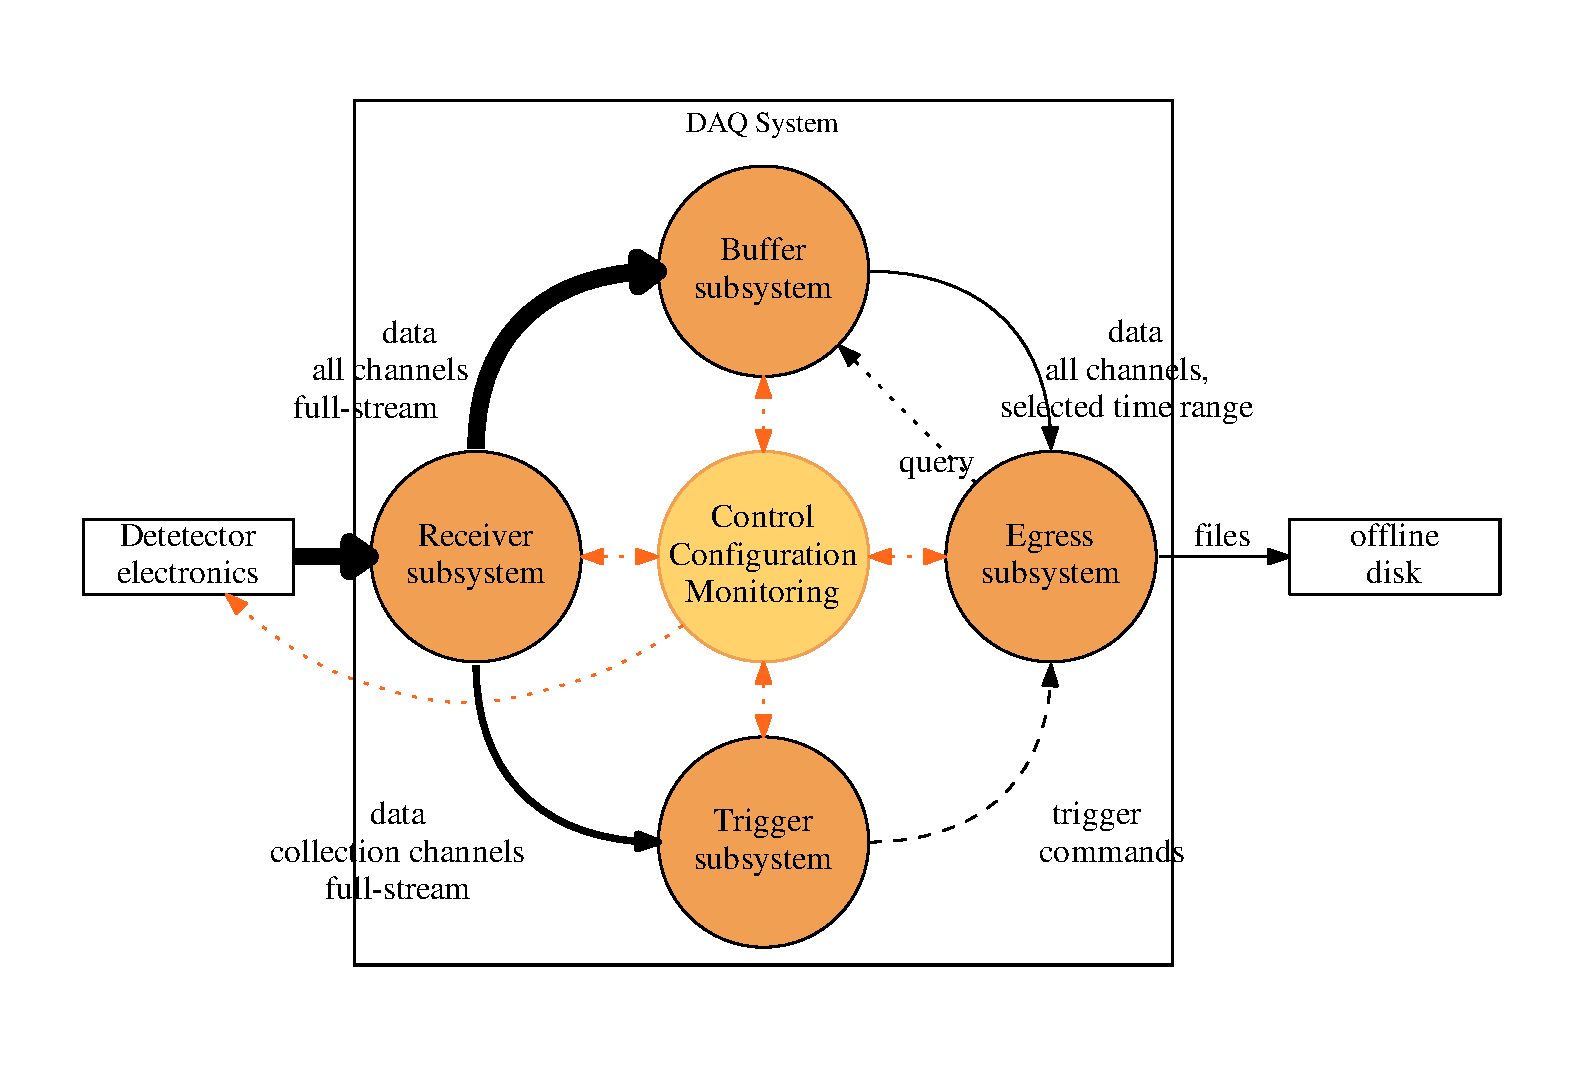
\includegraphics[width=0.8\textwidth]{daq-toplevel-conceptual.pdf}
\end{dunefigure}

These conceptual units are mapped to specific \dword{daq} subsystems as follows:


\begin{itemize}
%\item The data is input by the \dfirst{daqros} where it is buffered (see Section~\ref{sec:daq:design-readout}).
\item The \dfirst{daqros} inputs the data and buffers it (see Section~\ref{sec:daq:design-readout}).

\item A substantial portion of this data then flows into the \dfirst{daqdss}, which is the majority portion of the \dfirst{daqtrs}. This results in a stream of \dwords{trigcommand} (see Section~\ref{sec:sp-daq:design-selection-algs}).

%\item These commands are executed by the \dfirst{daqbes} by querying the buffers for the selected data, aggregating the results and output that as files on nonvolatile stores which then become custody of the DUNE offline (see Section~\ref{sec:fd-daq:design-backend}).
\item The \dfirst{daqbes} executes these commands. It  queries the buffers for the selected data, aggregates the results, and outputs the results as files on nonvolatile stores. The files then become custody of offline computing (see Section~\ref{sec:fd-daq:design-backend}).


%\item Pervasively, the central orchestration is provided by \dfirst{daqccm} (Section~\ref{sec:fd-daq:design-run-control}), overall communication by the \dfirst{ipc} subsystem (Section~\ref{sec:daq:design-ipc}) and synchronization is provided by the \dfirst{daqtss} (Section~\ref{sec:sp-daq:design-timing}).
\item Pervasively, the  \dfirst{daqccm} provides the central orchestration (Section~\ref{sec:fd-daq:design-run-control}), the \dfirst{ipc} subsystem provides overall communication (Section~\ref{sec:daq:design-ipc}), and the \dfirst{daqtss} provides synchronization (Section~\ref{sec:sp-daq:design-timing}).
\end{itemize}


%In addition to deconstructing the design into subsystems, the \dword{daq} is also separable into multiple \dwords{daqpart} or instances.
In addition to deconstruction of the \dword{daq} design into subsystems, it is also separable into multiple \dwords{daqpart} or instances. 
Each partition 
\fixme{how does daqpart or instance relate to`partition'? anne} services some set of detector electronics. 
A partition may span an entire %up to one
 \dword{detmodule} or some subset of its electronics. 
A distinct partition will %also be employed for the validating of 
validate detector electronics and hardware during installation and commissioning as described in Section~\ref{sec:sp-daq:production}.
Partitions may operate wholly independently from one another, or be loosely coupled through trigger commands.  
%More description of the nature of partitions may be found 
This is further described in Section~\ref{sec:daq:partition-lifetime}.



\metainfo{For the remaining design sections: do not include directly validation info but rather place this information in Section~\ref{sec:sp-daq:design-validation} and make references.}
  



\subsection{Inter-process Communication}
\label{sec:daq:design-ipc}
\fixme{module-generic}

The \dword{daq} must transfer data between external sources and elements inside the \dword{daq}. 
These data are characterized using a variety of schema, latency, and throughput. 
The system that provides for such transfers is generally termed \dfirst{ipc}.
An \dword{ipc} system consists of the following elements:
a set of message types, their data formats and schema,
a high-level application protocol that governs the exchange of its messages,
a set of supported message transport mechanisms, and
behavioral expectations for the participants in the message exchange. 


For the most part, the \dword{fd} \dword{daq} will require that supported transport mechanisms be \textit{reliable}, where 
reliable means that when one endpoint sends a message,
% that it shall be received by 
the other endpoint shall receive it even in the case of temporary loss of network connectivity or %possibly 
temporary termination of the receiving endpoint.
The acceptable duration the broken connectivity is chosen based on the particular protocol in use.
Related to reliability, an \dword{ipc}  system may also provide behavior such as the \dword{daqdispre} function described in Section~\ref{sec:fd-daq:design-run-control}.

By design, \dword{ipc} is a system that interconnects diverse components and thus can encompass substantial complexity. 
%In order 
To manage complexity and for practical reasons, the overall \dword{ipc} system is segmented into a number of \dword{ipc} domains. 
In fact, 
\fixme{are we trying to say ``This accommodates certain... that may require their own...? anne}
certain \dword{daq} subsystems may require their own unique \dword{ipc} implementation.
The \dword{daq} consortium will develop a single inter-domain \dword{ipc} system %will be developed 
for the \dword{fd} \dword{daq} 
%This system will 
to provide a global \textit{lingua franca} communication between the domains. 
Some domains will also use this \dword{ipc} for internal communications. 
We will also develop a proxy service component %will be developed
 to translate between the \textit{lingua franca} \dword{ipc} and any domain that utilizes a unique \dword{ipc} system.

The \textit{lingua franca} \dword{ipc} will be chosen after identifying options and evaluating them in terms of their features, performance, documentation and development simplicity. 
The selected \dword{ipc} should also provide %have an expectation of
 long-term and broad open source community support. 
The current candidate for a basis of the \textit{lingua franca} \dword{ipc} is ZeroMQ\footnote{The reference for ZeroMQ, Zgossip, and Zyre is \url{http://zguide.zeromq.org/}.},
which CERN~\cite{Dworak:2012mf} evaluated positively. 
ZeroMQ provides a well established, high-performance library. 
%It has been positively evaluated by 
It provides the basic building blocks for an \dword{ipc} system in the form of high-level socket objects implementing a variety of socket patterns including publish/subscribe, exclusive pair, request/reply, and others. 
Messages may %be transported across 
traverse thread-safe queues, Unix domain, and network sockets. This greatly assists in developing elastic applications that can scale from multi-threaded, multi-process and multi-computer contexts merely by changing configuration. 
The ZeroMQ ecosystem includes higher-level libraries providing for such important features as distributed discovery and presence (Zyre) as well as distributed configuration databases (Zgossip). 
Finally, it provides securely authenticated and authorized connections through elliptic curve public key encryption, which will be useful for protecting some key communication against inadvertent connections. \fixme{``key communication'' = communication of the encryption key or = critical communication? anne}

One example of a subsystem likely to utilize the \textit{lingua franca} \dword{ipc} directly is the hierarchical trigger processing system provided by \dword{daqdsn} (Section~\ref{sec:sp-daq:design-selection-algs}).
An example of a domain-specific \dword{ipc} is that used by \dword{artdaq} that will be the heart of the \dword{daqbes} %as 
described in Section~\ref{sec:fd-daq:design-backend}.
The \dword{daq} will also interconnect with external domains. 
For example, a two-way exchange of information will exist between \dword{daq} and \dword{cisc}, as described in Section~\ref{sec:sp-daq:interfaces-cisc}.  

The \dword{daqccm} subsystem (Section~\ref{sec:daq:design:ccm:control}) must communicate with all \dword{daq} domains and in some cases directly to domain components. It is therefore % and so is 
also expected to use the \textit{lingua franca} \dword{ipc}. 
As described in that section, some of its functionality, particularly that of discovery, presence and zero-downtime reconfiguration, places requirements on the \dword{ipc}.

\fixme{need references fo zeroMQ, zgossip zyre, artdaq. email to bv, gk sent}

\subsection{Control, Configuration, and Monitoring}
\label{sec:fd-daq:design-run-control}
% \fixme{module-generic}

% \metainfo{Describe run control and \dword{daq} operation monitoring. 
%   How it makes use of the Message Passing System. 
%   What is an ``epoch''.
%   How Epoch Change Requests lead to zero downtime reconfiguration. 
%   Public key based ``iron'' authentication between run control processes and the controlled processes. 
%   Describe how RC will configure partitioning, initiate reconfiguration, handle ``run'' changes, node discovery, configuration, logging, startup, shutdown and failures are handled. Describe how RC will support detector electronics configuration.}

The \dfirst{daqccm} subsystem, illustrated in Figure~\ref{fig:daq-ccm-subsys}, encompasses, as its name suggests, the software needed to control, configure, and monitor the rest of the \dword{daq}, as well as itself. 
It provides a center for the highly distributed \dword{daq} components, allowing them to be treated and managed as a coherent system. 
The \dword{daqccm} scope is high level in the sense that it does not directly handle the selection or transport of primary detector data but rather it handles (via \dword{ipc}, see Section~\ref{sec:daq:design-ipc}) the subsystem components that provide these functions.
Figure~\ref{fig:daq-conceptual-overview} shows the central role of the \dword{daqccm} within the complete \dword{daq} system.
The following sections describe the \dword{daqccm} subsystems. 

\begin{dunefigure}{fig:daq-ccm-subsys}{Main interaction among the three \dword{daqccm} subsystems.}
  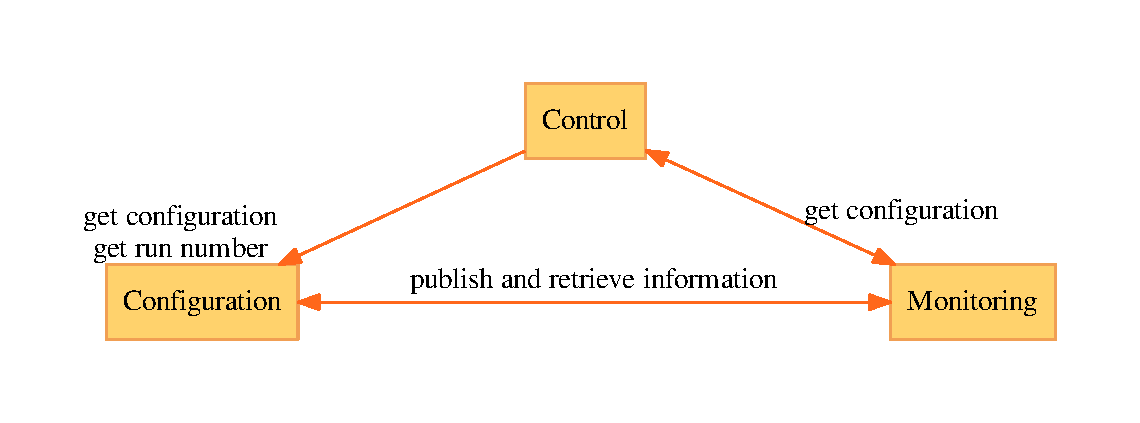
\includegraphics[width=0.8\textwidth]{daq-ccm-subsys.pdf}
\end{dunefigure}

\subsubsection{Control}
\label{sec:daq:design:ccm:control}


The \dword{daq} control subsystem actively manages \dword{daq} software process lifetimes, asserts access control policies, executes commands, initiates configuration changes, detects and handles exceptions, and provides an interface for human operators.

% \fixme{I (bv) redrew this from Giovanna's to get vector PDF and match \dword{dune} color palette.  I made two content changes: 1: move UI out of partition as it can't both initiate a partition and be inside it and likely will allow for creation/viewing of more than just one partition.  2: I had to guess on how garbage collection might go and so addded a line from RM to PM. }

\begin{dunefigure}{fig:daq-ccm-control}{Roles and services that compose the \dword{daq} control subsystem.}
  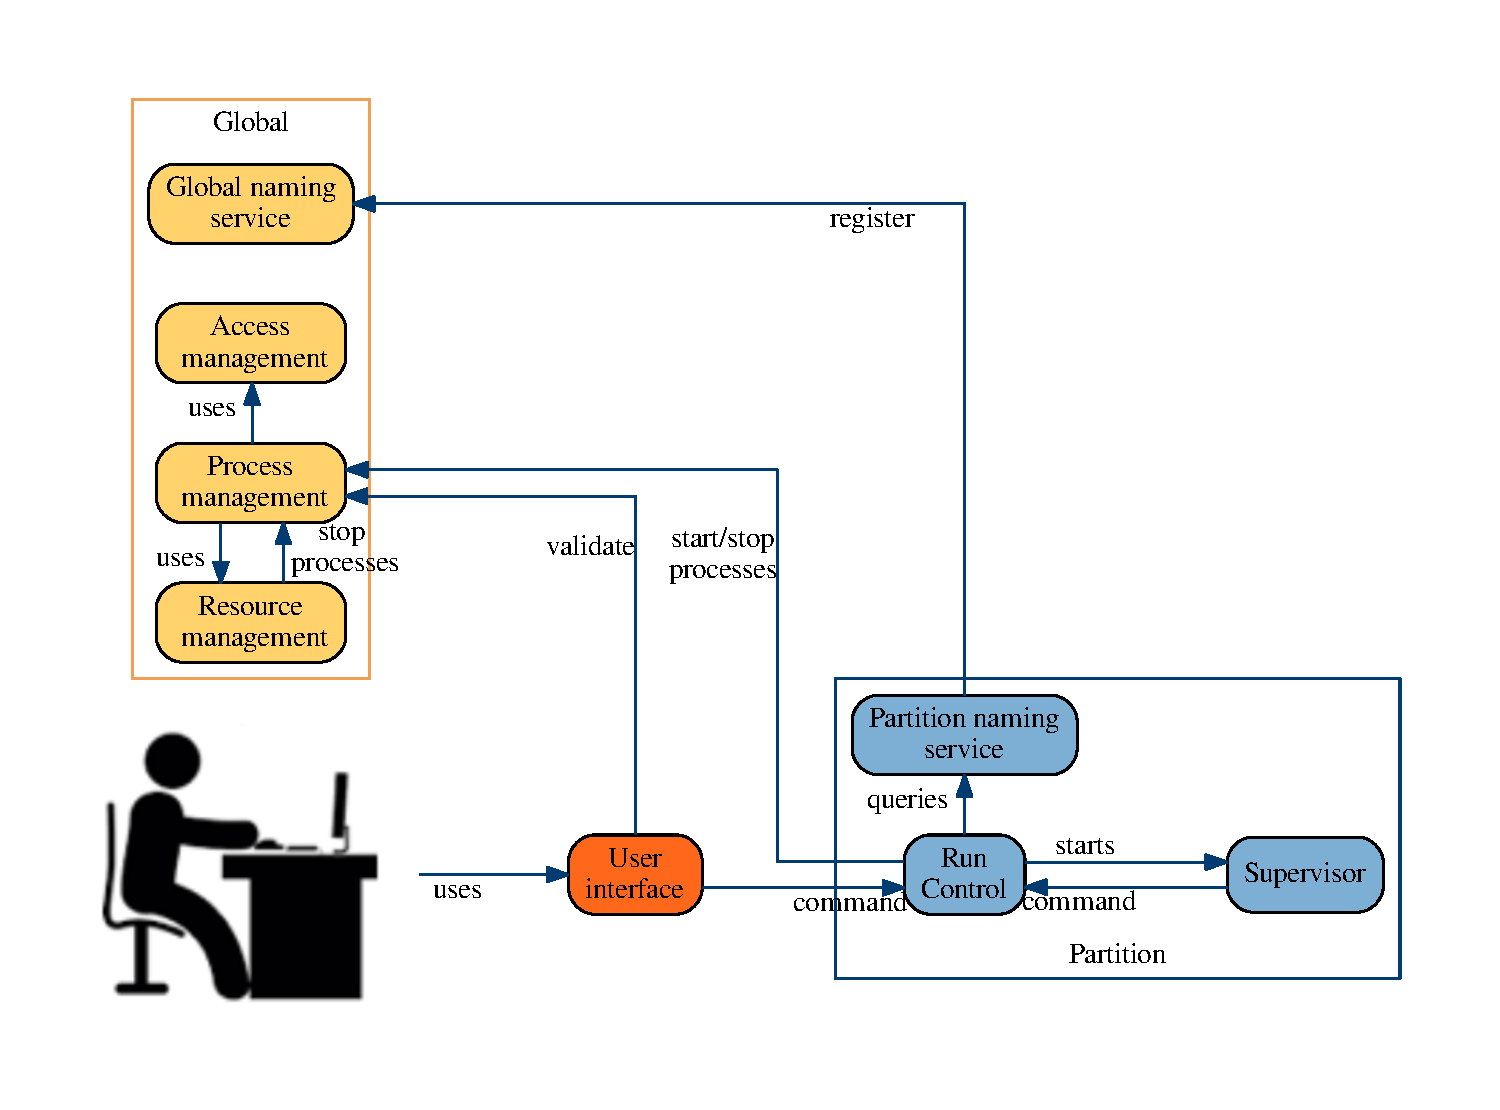
\includegraphics[width=0.8\textwidth]{daq-ccm-control.pdf}
\end{dunefigure}

The control subsystem comprises a number of functional blocks of either global or partition scope as illustrated in Figure~\ref{fig:daq-ccm-control}. 
In the figure, ``partition'' refers to a logical segmentation of the \dword{daq} where each segment operates to some extent independently from others. 
The segmentation applies to the portion of detector electronics that provides input to the partition's \dword{daqdsn} and readout. 
The largest partition %would be 
is that of one \dword{detmodule}. 
The functional blocks in the figure represent one or more semi-autonomous agents, each with defined roles, capabilities, and access. 
Although drawn as single blocks, they are each implemented as multiple peer agents to assure redundancy and fail-over. 
The blocks at partition scope are first described.

\begin{itemize}
\item Partition naming service provides \dword{daqdispre} for the components of a \dword{daqpart}. 
  That is, it allows a component to be made aware  of the creation and continued operation of other components (discovery) or that other components have recently become unresponsive (presence). 
  This service may be provided via distributed \dword{ipc} mechanism or by an explicit, centralized (but redundant) service.

\item Run control provides a central director;  its creation is the first step in initiating a \dword{daqpart}. 
  The \dword{rc} accepts, interprets, and validates input commands that may come either from a human via a user interface, or from other blocks. 
  The commands describe a desired state of the aggregate of all components that comprise the \dword{daqpart}. 
  \dword{rc} may query other blocks to validate commands and then execute the commands by allocating processes through process management. 
  Once successfully allocated, their lifetimes are managed by \dword{rc}. 
  Throughout its lifetime, \dword{rc} may reconfigure an existing process, destroy it, or allocate additional processes. 
  \dword{rc} may query the partition-naming service in order to resolve resource identifiers in commands into their corresponding network endpoint addresses.  

\item Supervisor provides a locus of expert system automation. 
  This block is initiated along with its \dword{rc} peer and augments human commands with automated ones. 
  For example, as certain ``common exceptions'' are encountered and understood so that a means to correct them can be developed, the supervisor can be extended to automatically issue the corrective actions that must otherwise be manually performed by a human operator.

\end{itemize}

Global scope controls \dword{daq} components for all \dwords{daqpart} across all \dwords{detmodule}\footnote{\dword{daq} instances at locations other than the \dword{fd} cavern are expected to operate in a wholly distinct manner.}.  It consists of the following blocks:


\begin{itemize}
\item Global naming service aggregates the \dword{daqdispre} information across partitions.  Like the partition naming service, this may be implemented as a centralized (but redundant) explicit service or may be provided by extending the IPC \dword{daqdispre} mechanism to the entire FD \dword{daq} network.

\item Process management allocates and may reclaim sets of processes on behalf of a requesting component (specifically \dword{rc} and resource management). 
  An allocation request includes a complete description of the processes and their desired initial configuration. 
  A successful allocation occurs only after this role successfully initiates all requested processes and confirms their presence. 
  Process management only allocates processes if their requester has appropriate access privileges as determined by access management and if resource management determines sufficient resources exist. 
  Process management may support pre-allocation if sufficient access and resources are confirmed and reserved; if so, a token (aka ``cookie'') is returned to the requester. 
  This cookie may be subsequently be presented to complete the allocation and claim the processes. 
  After a configured timeout, the cookie may be invalidated.\footnote{This will be required if the race condition between multiple UIs and RCs is a problem.}  
  
\item Resource management determines whether any process allocation can proceed and enacts a process garbage collection mechanism. 
  An allocation is successful if sufficient process resources are available and if it is consistent with a set of configured constraints maintained by this component. 
  Resource management monitors all allocated processes as well as the process initiating a request in order to perform ``garbage collection''. 
  This is performed in the event that the allocated processes outlive the requesting processes.
  Resource management  notifies process management of any remaining processes from an allocation when it detects that the requester is no longer present.
  Resource management also supports pre-allocation validation queries. 
  A validation response merely indicates current state and it represents no guarantee that the allocation will subsequently succeed.

  
\item Access management is responsible for providing authentication and authorization for all \dword{daq} functions that require access control. 
  This block may be implemented as an explicit centralized (but redundant) service or through a distributed IPC mechanism or as some mixture of the two designs. 

\end{itemize}

The last block in Figure~\ref{fig:daq-ccm-control} represents applications that provide user interfaces (UI) to the control subsystem.
At least one UI will be developed to allow a trained operator to construct and issue commands required to initiate, configure, potentially reconfigure, and finally terminate \dwords{daqpart}. 
The UI may validate user commands before issuing them to an \dword{rc} by directly querying the process manager block. 
If sufficient resources are unavailable or if the user lacks appropriate access privileges, the UI will present a descriptive error message or otherwise disable corresponding functionality.  
If the user permission is valid the UI sends the use-initiated command to the \dword{rc} for execution.
Note that subsequent commands from the \dword{rc} to other blocks are also subject to access management.
Additional UI elements will be developed as described in sections~\ref{sec:daq:design:ccm:configuration} and~\ref{sec:daq:design:ccm:monitoring}.


\subsubsection{Configuration}
\label{sec:daq:design:ccm:configuration}

The \dword{daq} configuration subsystem provides persistent data storage for all historic, current, and future configuration information applicable to the \dword{daq}.
Further, it will provides a singular (but redundant) service for the allocation of unique and monotonically increasing \dwords{daqrunnum}.
The configuration data stores are operated in an insert-only mode. 
They do not support updating nor deleting previous records.
Configuration subsystem  shall support storing the following types of information:

\begin{itemize}

\item Partition structure contains descriptions of the multiplicity and connectivity of \dword{daq} components for any partition. 
  Structure and connectivity is expressed in an abstract manner with logical addressing and not through concrete addressing (eg, host computer network address and port numbers). 
  This allows for identical structure to be reapplied to various collections of specific hardware.\footnote{It is the discovery and presence from naming services as described in Section~\ref{sec:daq:design:ccm:control} that allow mapping from abstract to concrete addressing.}

\item Component parameters comprise configuration information associated with any given \dword{daq} component.  This data is structured following a schema defined by the associated component and this schema is versioned to allow for schema evolution.

\item Run number provides a monotonically increasing sequence of \dwords{daqrunnum} that are allocated upon request to assure that each is unique.

\item Partition instances associate a \dword{daqrunnum} and the set of component parameters that were used to initiate a \dword{daqpart} or which are used to reconfigure an existing \dword{daqpart}.  

\item Constraints define rules that must be held true by resource management servicing requests for process allocations.  This information store also includes which constraints were used by resource management over time.
\end{itemize}


All storage provided by the configuration subsystem must provide assurances availability and integrity. 
This includes redundant storage hardware elements to allow for fail-over as well as copies made and stored off-site and with a mechanism for their restoration if catastrophic data loss occurs.
Certain configuration stores must assure additional requirements such as those on \dword{daqrunnum} allocation mentioned above.

Access to the configuration store by a client application should be through a generalized intermediate layer and not via a mechanism that ties the client application to the particular storage software technology and performance.

Configuration editors and generators will be developed to produce and store data structures that are too complex for manual construction. 
They enable expert operators to construct wholly novel configuration and produce variants based on existing structures.

\subsubsection{Monitoring}
\label{sec:daq:design:ccm:monitoring}

The \dword{daq} monitoring subsystem will help both humans and expert systems in detecting, diagnosing, and correcting anomalous activity, observing intended operation, and providing a historical record.
This subsystem will accept required information produced by any \dword{daq} component (here called status).
Status shall be stored for not less than what is required for the corresponding detector data to be validated in an initial offline data quality validation procedure.
Status must be in a form that humans can understand with only minimal processing and delay. 
The definition of promptness requires further study to identify the required latency. This is expected to vary depending on the type of status and its purpose.  
The monitoring store will allow status to be retrieved based on when it was produced and the logical and physical addresses associated with its producer.
In addition, views will be produced that can display ``live'' status as it arrives via direct feeds from individual components.

The precise implementation of the production, acceptance, store, post-processing, querying, and visualization of monitored status requires additional work. 
However, the selected \textit{linuga franca} IPC system described in Section~\ref{sec:daq:design-ipc} will be used to deliver status information to the monitoring subsystem. 
Where this may conflict with a native IPC used by any subsystem, a proxy will be supplied. 

In general, the publish-subscribe (PUB/SUB) network communication pattern will be used to deliver status. 
The monitoring system may be further divided into a number high-level IPC protocols with message specified by their type, format and schema.
These are categorized as


\begin{itemize}
\item Common portion of messages include message type and instance identifier (count), a PUB/SUB topic, sender, the associated detector data time the recent host computer time.  Specific protocols extend this basis by providing additional payload to their messages, as described in the following items.
 
\item Logging messages add a an integer determining subjective importance (e.g., enumerating categories like debug, info, warning, error, fatal) and a succinct, human-readable information string explaining what led to the occurrence.
  
\item Metrics provide structured data carrying specific information about predefined aspects of the sender. 
  This is similar to logging, but the messages support automated consumption by expert systems.  

\item Quality messages summarize information derived from the detector data (e.g., waveforms) or its metadata (e.g., timestamps, error codes) while that data is ``in flight'' through the \dword{daq}.

\end{itemize}

Some status feeds accepted by the monitoring subsystem may be processed so that only the resulting data is sent to permanent storage. 
In particular, the quality stream data rate may be prohibitive of long term storage in forms that meet the query requirements given earlier. 
This stream may be summarized into histograms or other statistical representations that will be saved.
Such high rate streams may be then discarded or saved in some other form for archive purposes.

In addition to this \dword{daq} \dword{daqccm} monitoring subsystem, a separate system must be used to monitor the quality of the detector data content itself.  See Section~\ref{sec:fd-daq:design-data-quality} for the description of this data quality monitoring system.

\subsubsection{Partition Lifetime}
\label{sec:daq:partition-lifetime}

The partition lifetime is described here in a somewhat linear narrative, it should be noted that the components will be constructed through some suitable protocol that need not progress in the same linear order. 
In particular, the operation of the partition components shall be robust to the order in which peers are discovered.

After a process is executed via the allocation mechanism described in Section~\ref{sec:daq:design:ccm:control}, it will apply its initial configuration. 
This information includes any personal identifiers the component will assert as part of \dword{daqdispre} as well as any identifiers required to find any other peer components which are needed for its own operation. 
In particular, a component is provided the identity of the partition's \dword{rc} instance so that it may receive control directives.

It is through a control directive enacted by each individual component that the overall partition structure and connectivity emerges.  
These directives must be issued prior to some activation criteria in order to enable the \textit{zero-downtime reconfiguration} feature as described next.
The control directive contains a \dfirst{ccc}.
A \dword{ccc} provides, at a minimum, the following pieces of information:

\begin{itemize}
\item Run number is as described in Section~\ref{sec:daq:design:ccm:configuration}. 
  Here, it identifies a desired and collective partition state which will be constructed once all \dwords{ccc} are enacted.
\item Activation time stamp (ACT) states the \textit{data time} (see Section~\ref{sec:daq:design-ipc}) at which the \dword{ccc} shall take effect. 
\item Configuration payload provides the component-specific configuration to be enacted and may include   actions must be performed prior to the \dword{act} in order to assure a zero-downtime transition.
\end{itemize}

When a \dword{ccc} is received by a component, that component initiates any new connections with peers and performs any other pre-\dword{act} actions as directed by the \dword{ccc}. 
The component then begins (or continues) to monitor the \textit{data time} of received messages on its new (or previous) input sockets. 
If the component was operating as part of the prior partition it will continue to service its previous input and produce output to any previously connecting consumers.
Data is not yet sent to any new connections.
Upon receiving input with a data time after the \dword{act} it will apply the new configuration specified in the \dword{ccc}. 
In this reconfiguration process, any pre-\dword{act} data that may still be buffered by the component shall be flushed to its (previously connected) output sockets. 
Any input or output connections no longer applicable to the new, post-\dword{act} partition definition shall be dropped. 
Finally, the component shall renew operations, beginning with the held data which had satisfied the \dword{act} criteria and which initiated the reconfiguration processes.

For this mechanism to truly provide zero-downtime, the partition components must receive reconfiguration messages from the \dword{ccc} sufficiently in advance of input data passing the \dword{act}.
This means the human-UI-\dword{rc} chain must select an \dword{act} knowing the most recent \textit{data time} as well as some lead time to apply.  
For any given reconfiguration an optimal lead time involves many interdependent factors but may be estimated by considering a maximum calculated over all components involved in the reconfiguration of the time difference between their required reconfiguration time and the latency for data to arrive at the component from the time of sampling. 
In a real system this maximum has some distribution. 
In practice it is expected that the lead time must be chosen in some %empiric 
manner or simply ``long enough''.
Even a generous choice is likely to satisfy human human impatience especially given the alternative is accepting data loss.

Although the lead time may need to be many seconds, it is important to note that the minimum time between subsequent \dword{act}s is essentially zero. 
Multiple sets of \dwords{ccc} may be issued over some short time span and queued by components. 
In principle, this allows zero-downtime sequencing of runs of arbitrarily short duration.
Practically however, this may be limited due to performance issues. 
For example, if a new set of \dwords{ccc} requires many duplicate readers of data streams this may cause bandwidth limits to be reached. 
To the extent this fast run sequencing is needed, these potential limitations require additional study.

Finally, after cycling through one or more run numbers, the partition may be terminated. 
A final round of \dwords{ccc} is issued by the partition's \dword{rc}. 
Each \dword{ccc} directs the termination procedure of its component. 
This procedure starts just as any zero-downtime reconfiguration. 
The \dword{ccc} instructs the component to continue processing until receiving input data which satisfies the \dword{act} criteria at which time any remaining buffered data is flushed to the component output connections. 
Then, unlike zero-downtime reconfiguration, the component simply destroys all connections and exits. 
The \dword{rc} notifies the UI and process manager of the destruction of the partition (saving, for the moment, the destruction of the \dword{rc} itself). 
The process manager notifies the resource manager that the resources have been released. 
The \dword{rc} then terminates itself, and the partition is no more.
The resource manager confirms partition processes have terminated through \dword{daqdispre}. 
In the odd case that the \dword{rc} aborts without cleanly terminating the partition, its absence must be detected, and the remaining partition processes are reaped in the garbage collection mechanism described in Section~\ref{sec:daq:design:ccm:control}.

\subsubsection{Self-healing}
\label{sec:daq:self-healing}

The above zero-downtime reconfiguration mechanism is intentional and typically driven by human action or automated run sequencing algorithms. 
Similarly, the partition will be \textit{self-healing} in the face of unexpected failures that render peers unresponsive or when unexpected information content is received by partition components.  
Extending the metaphor, self-healing involves these phases: \textit{detection} of an injury to the partition, \textit{diagnosis} of the scope of the injury, and \textit{intervention} that executes an action on the partition.

Detection is performed by the \dword{daq} control subsystem supervisor functional block using at least one of two methods.
First, if a component in the partition becomes unresponsive (i.e., it crashes or hangs) the supervisor  receives notification through \dword{daq} \dword{daqdispre}. 
Second, if a component directly detects injury, such as may be the case when it receives  data outside of expected norms, it reports this fact through \dword{ipc} to the supervisor.

When injury is detected the supervisor  diagnoses this using heuristics and other methods that are expected to evolve as failure modes are discovered or removed. 
It is thus crucial that the supervisor is designed and developed in a way that facilitates this ongoing evolution.  

Finally, the supervisor responds to the diagnosis with some intervention. 
Response  in all cases includes notifying the monitoring subsystem. 
Any additional response involves sending commands to the \dword{rc} to initiate a reconfiguration,  which may be to terminate the partition.
When initiating a reconfiguration, as with any reconfiguration, the command to the \dword{rc} must include information required by the \dword{rc} to issue \dword{ccc} messages. 
If the partition remains it is reconfigured and thus begins a new run number as described in Section~\ref{sec:daq:partition-lifetime}.


\subsection{Detector Readout}
\label{sec:daq:design-readout}
%\fixme{module-generic}

The readout provides the first link in the data flow chain of the \dword{daq} system.
It provides the input to which the data from detector electronics flow.
It implements a receiver, buffer, and a portion of the trigger concepts illustrated in Figure~\ref{fig:daq-conceptual-overview}.
It is physically connected to the detector electronics via optical fiber and buffers and serves data to other \dword{daq} subsystems, namely the \dword{daqdsn} and the event builder as detailed in Figure~\ref{fig:daq:readout}.

\fixme{It would be nice to redraw this using \dword{dune} colors.}

\begin{dunefigure}{fig:daq:readout}{\dword{dune} \dword{daq} readout system and its connections.}
  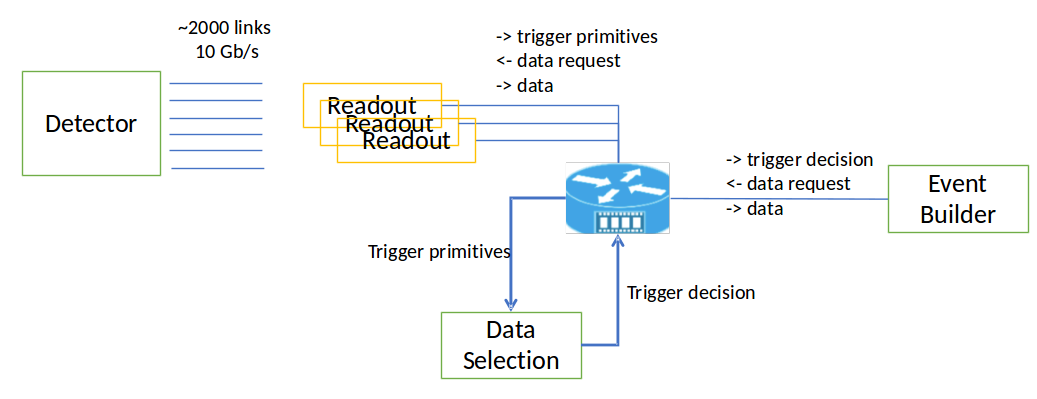
\includegraphics[width=0.8\textwidth]{daq-readout.png}
\end{dunefigure}

The readout system comprises many similar \dword{daqrou}, each connected to a subset of electronics from a detector module and interfacing with the \dword{daq} switched network.  Each unit encompasses four functional blocks:

\begin{enumerate}
\item Data reception
\item Network based I/O
\item Data processing
\item Temporary data storage
\end{enumerate}

Each of these blocks is described below.  In addition, and like all other \dword{daq} subsystems, the readout participates in the common software framework for control, configuration, and monitoring as described in Section~\ref{sec:fd-daq:design-run-control}.

\subsubsection{Data reception}

The physical interface between the detector electronics and the \dword{daq} to transmit data consists of 10 Gbps point-to-point serial optical links, running a simple (e.g., 8/10 bit encoded) protocol. 
The number of links per \dword{dune} module varies from approximately 1000 to 2000, depending on the detector technologies adopted.

To minimize the space and power consumption footprint of the \dword{daq}, 10-20 links are aggregated into \dword{felix} boards hosted in commercial, off-the-shelf computers.
\dword{felix} is an \dword{fpga}-based PCIe board developed initially for ATLAS and now proposed or already used in several experiments, including \dword{protodune}. 
Existing firmware will be adopted and adapted to ensure decoding and format checking of incoming data and then to marshal the data to other blocks of the readout subsystem.

\subsubsection{Network based I/O}

The readout system provides access to the \dword{daqdsn} and \dword{daqbes} through a commercial, off-the-shelf switched network as illustrated in Figure~\ref{fig:daq:readout}).
The network communication protocol is as described in Section~\ref{sec:daq:design-ipc}.
The network I/O is handled by the \dwords{daqrou} via software; dedicated hardware or firmware development is not required.

\subsubsection{Data processing}

The data processing functional block identifies active areas in the detector (in the TPC and photon detection systems) as a function of time.

As a preliminary step, data may be pre-processed, i.e., organized however best suits subsequent data analysis. This implies reorganizing data into different streams, applying noise filtering algorithms, and compressing or zero-suppressing data.

The readout system summarizes the identified detector activity (``hit finding'') on a per-channel basis into information packets called \dwords{trigprimitive}.  These are forwarded to the \dword{daqdsn} system which makes correlations and decides whether and which data is to be saved.

This functional block may be implemented onto FPGAs, GPUs, CPUs, or a mixture of these elements.
Deciding on the implementation is premature at this stage; this is one of the main topics to explore and develop in the readout area.

\subsubsection{Buffering}

In \dword{dune}, the readout system is in charge of buffering all detector data until the \dword{daqdss} has formed a trigger decision (Section~\ref{sec:sp-daq:design-selection-algs}) and until the \dword{daqbes} (Section~\ref{sec:fd-daq:design-backend}) may have sufficient time to request and receive that selected data. 
In addition, a small portion of the data must be buffered for much longer to absorb the strongly punctuated bottlenecks that form when the \dword{daqdss} observes a potential \dword{snb}.
There are two rather different time scales and data throughput metrics which must dictate the technology and the scaling required for the temporary storage providing the buffering.
As described in Section~\ref{sec:sp-daq:design-selection-algs} these are due to localized and extended activity.

The buffering time required to select data containing localized activity is dominated by processing speed, pipeline depths and network latency. 
Some studies must still be performed but initial estimates indicate that the time buffering time required is should not exceed a maximum of approximately one second. 
The amount of data that must copied from buffering in order to capture the localized activity is expected to be one or two TPC drift times (5-10\si{\milli\second}), depending on detector technology).
As the full stream of data must constantly be buffered, a RAM technology is selected based on providing sufficient throughput, endurance, and capacity.

The extended activity (e.g., due to a potential \dword{snb}) presents a far more challenging set of buffering requirements.  
Extended activity that is below triggering threshold may exist for as much as \snbpretime prior to it increasing in rate such that the trigger criteria may be satisfied. 
This below threshold activity may be extracted using more sophisticated and processing intensive algorithms if the data can be recorded. 
A second challenge in recording data containing extended activity is that all channels must be recorded for as much as \snbtime around its trigger time.
This can require extracting as much as \spsnbsize.
It is not cost effective to design the \dword{daq} with a full path to final output that can accept this rate pulse.
Thus, bottlenecks must be allowed and additional buffering provided to catch the temporary backlog the pulse will produce.

The technology and scale of this additional buffering must satisfy several requirements. 
It must accept the full data rate of the detector (as much as \SI{2}{\tera\byte/\second}). 
The data must then reside on nonvolatile media. 
The media must have sufficient capacity and allow for sufficient extraction throughput so that it is vanishing unlikely to be allowed to become too occupied to accept another pulse of data. 
For planning purposes it is assumed that, on average, a \dword{snb} trigger condition will be satisfied once per month. 
Statistically, this may fluctuate to twice per day only about once every decade.
Given this, and costs, clearly the  best technology is %the use of 
solid-state devices, which at the scale required to provide suitable input bandwidth, can provide a capacity to write the data from several extended activity triggers.
Providing only a modest overhead to normal operations, this data can be extracted from such storage from the \dword{daq} in under a day.

For both types of activity, the buffering requirements may be reduced by employing lossless compression to the data prior to it entering the buffer.
This can be expected to provide at least a factor of two reduction in buffer input rate. 
If expected noise levels are achieved this compression would provide a factor of four to ten, depending on the detector module technology.
Effort is currently underway to understand the costs and technology involved in exploiting this benefit.


% \ifdp
% \subsubsection{DP data ingest via UDP}
% \label{sec:dp-daq:design-udp-ingest}
% \fixme{dual-phase module, move to DP \dword{daq} chapter eventually}
% \metainfo{This is a DP section and will be only in the DP volume. 
%   It should describe the ``Bump On Wire'' from the IDR unless we can
%   come up with any new/better ideas.}
% \metainfo{Include full hardware scope starting at fibers from CE and
%   ending at the output of trigger processors and the interface between
%   buffer and the Data Selector.
%   Describe the per-APA multiplicity of computers, CPU cores, host
%   system RAM, host system storage,  \dword{felix}  boards, DPM components (RAM,
%   SSD). 
%   Include thermal estimates itemized by components.}  
% \fi

% \subsection{Front-end Data Handling and Processing}
% \label{sec:sp-daq:design-fe-processing}

% \metainfo{This section describes four functional blocks: (1) 10s RAM buffer (minimum), (2) non-volatile SNB buffer for 30s of data once per month (minimum), (3) hardware for the production of trigger primitive including any data formatting and DPS filtering and (4) compression of selected data.  Note, actual algorithms for trigger primitives are described in Section~\ref{sec:sp-daq:design-selection-algs}.}

% \metainfo{One or two sentences that positions the two processing
%   patterns (FEDHP either before or after  \dword{felix} ) in this section as options. 
%   Say that the ``FPGA before  \dword{felix} '' option is used for ``baseline costing''.}

% \metainfo{Include a table with one row for each known compression factor: \dword{protodune} RCE and  \dword{felix} , MicroBooNE before and after noise filter (see docdb), 35t, \dword{protodune} data after \dword{adc} stuck code mitigation or avoidance, simulations.  One column of this table shall give a brief comment of how it applies to \dword{dune} including any caveats or reasons for over/under estimation.}

% % \subsubsection{ \dword{felix} +FPGA}
% \subsubsection{Upstream FPGA and Firmware}
% \label{sec:sp-daq:design-felix-fpga}
% \fixme{single-phase module}

% \metainfo{Include full hardware scope starting at fibers from CE and
%   ending at the output of trigger processors and the interface between
%   buffer and the Data Selector.
%   Describe the per-APA multiplicity of computers, CPU cores, host
%   system RAM, host system storage,  \dword{felix}  boards, DPM components (RAM,
%   SSD). 
%   Include thermal estimates itemized by components.}

% % \subsubsection{ \dword{felix} +CPU}
% \subsubsection{Downstream CPU and Software}
% \label{sec:sp-daq:design-felix-cpu}
% \fixme{single-phase module}

% \metainfo{Include full hardware scope starting at fibers from CE and
%   ending at the output of trigger processors and the interface between
%   buffer and the Data Selector. 
%   Describe the per-APA multiplicity of computers, CPU cores, host
%   system RAM, SSD and  \dword{felix}  boards. 
%   Include thermal estimates itemized by components.}


% \subsubsection{Photon Detection System Interface}

% \metainfo{Some motivations for using light to trigger. 
%   (1) want to understand PDS so want to trigger on just the PDS. 
%   (2) background to SNB for which PDS trigger primitives may eliminate. 
%   (3) possibly must rely on light only for SNB triggering, eg if noise is out of control. 
%   Some to all of these should be included.}

% \metainfo{Possibly want to \SI{1}{\micro\second} packet for every time a 1-PE threshold is crossed. 
%   PDS is still understanding what they may send. 
%   \dword{daq} needs to be in control of the trigger forming.}

% \ifdp
% \subsubsection{DP TPC FE issues}

% \fixme{dual-phase module}

% \metainfo{This is similar to SP except for the need to decompress before any trigger primitive processing.  Decompression can potentially happen on  \dword{felix}  FPGA or on CPU.  There shall be a table or description of the amount of processing required.}

% \subsubsection{DP SP Issues}
% \fixme{dual-phase module}
% \fi

\subsection{Data Selection}
\label{sec:sp-daq:design-selection-algs}
%\fixme{single-phase module}
%\fixme{There are many studies which could go into this section. Some of this may very likely be moved into one or more tech notes and referenced.}

The \dfirst{daqdss} is responsible for immediate and continuous processing of a substantial fraction of the entire input data stream. 
This includes data from TPC and PDS subdetectors.
From that input, the \dword{daqdss} must form a \dword{trigdecision},
which in turn produces a \dword{trigcommand}.
This command summarizes the observed activity that led to the decision
and provides addresses (in space and time) of the data in the \dword{fe} buffers that capture information about the activity.
This command is sent to and then consumed and executed by the \dword{daqbes} as described in Section~\ref{sec:fd-daq:design-backend}. 
It is also propagated to the \dword{etl} which may distribute it to other \dwords{detmodule} for consideration.

The pipelines of processing required for \dword{daqdsn} may execute in
various stages and forms using different firmware and software
implementations. 
Development is actively ongoing to demonstrate
viability and performance of different implementations. In satisfying
the philosophy and strategies of the \dword{daq} design there is 
flexibility in defining whether each element of a pipeline executes on
\dword{fpga}, CPU, GPU, or in principle, some other future hardware
architecture. 

The \dword{daqdss} must select data associated with beam interactions,
calibration signals, atmospheric neutrinos, rare baryon-number-violating events, and cosmic ray events that deposit visible energy in excess of 100 MeV, with high efficiency (targeted at $>$99\%). 
It must also select data associated with potential galactic \dfirst{snb}, indicating that the \dword{daqdsn} subsystem must be able to self-trigger on galactic \dword{snb} with galactic coverage\footnote{Galactic coverage is defined as efficiency-weighted probability of galactic \dword{snb}.} of $>$95\% efficiency.
To meet the requirement that the \dword{dune} \dword{fd} maintain a
$<$\SI{30}{\peta\byte/\year} to permanent storage, the \dword{daqdss}
subsystem must make \dword{daqdsn} decisions in a way that allows the \dword{daq} 
system to reduce its input data by almost four orders of magnitude
without jeopardizing the above efficiencies.

The \dword{daqdss} subsystem design follows a hierarchical structure, where low-level
decisions are fed forward into higher-level ones until a  module-level trigger is activated. The hierarchy
is illustrated in Figure~\ref{fig:daq:data-selection}. The structure
has three levels of \dword{daqdsn}: (1) low level trigger, which may consist of
\dword{trigprimitive} generation and subsequent
\dword{trigcandidate} generation; (2) module level trigger; and (3) \dword{hlt}. Each is trigger level described in subsequent
sections. An additional subsystem component is the external trigger,
which serves as a common interface for the
module level trigger of each of the FD \dwords{detmodule} and between
the module level trigger and other systems (e.g.,~calibration, beam
timing signals) within a single \dword{detmodule}.

\begin{dunefigure}{fig:daq:data-selection}{Block diagram of \dword{dune} \dword{daq}
    \dword{daqdsn} subsystem, illustrating hierarchical structure of
    subsystem design.}
  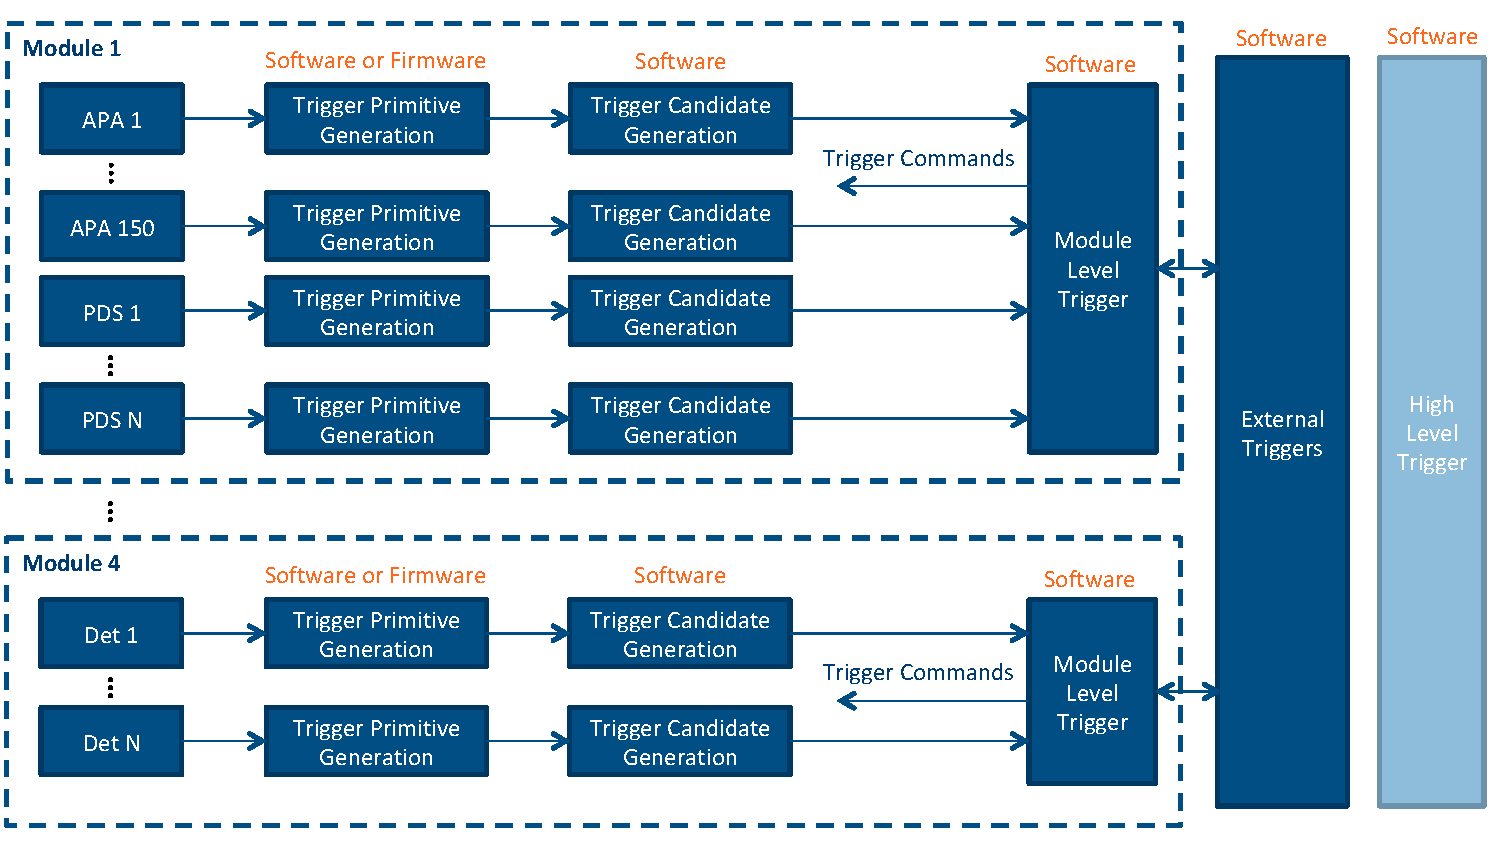
\includegraphics[width=0.8\textwidth]{DUNE_TDR_SP_DAQ_DS_Figure.pdf}
\end{dunefigure}

The first stage of DUNE FD operations will have two general classes of trigger
decisions that are categorized in terms of the distribution of activity
in time and space from which they are derived:
\begin{itemize}
\item Localized activity triggers are low-latency triggers intended to
  initiate the readout of high-energy events (depositing $>$100~MeV of
  visible energy). 
  They may also initiate the readout of low-energy events (e.g., from
  solar neutrino interactions).
  Data from all channels of the detector module and for a period
  spanning two drift times around the time of the localized activity
  trigger will be read out.\footnote{Strictly, all channels in the \dword{daq} partition.}
\item Extended activity triggers are high-latency
  (but no more than 10 seconds) triggers intended to initiate readout of
  activity associated with \dword{snb}. 
  Noticeable \dword{snb} activity is expected to span many tens of
  seconds and be comprised of a few thousand individual supernova
  neutrino interactions (eg in the case of a galactic \dword{snb}) which
  are spaced throughout the detector module and peaking over a time
  period of approximately ten seconds.
  When a module asserts an \dword{snb} trigger it is sent to the
  \dword{etl} and passed to other modules. 
  Regardless of its origin, a detector module will read out data which
  arrived \snbpretime prior to the trigger time and will read out a
  total of \snbtime data. 
  This data will be readout from all detector module electronics
  channels in both the PDS and TPC systems. 
  After sufficient confirmation of quality the \dword{snb} trigger will
  also be sent to global coincidence trigger recipients such as
  \dword{snews}.
\end{itemize}

To facilitate partitioning, the \dword{daqdsn} subsystem must also be
informed and aware of current detector configuration and conditions and
apply certain masks and mapping on subdetectors or their fragments in
its decision making. This information is delivered to the
\dword{daqdss} from the \dword{daqccm} system.

Ultimately, each \dword{trigdecision} culminates in a command sent to \dword{daqbes}. 
This command contains all the logical detector addresses and time ranges
required such that an \dword{eb} may properly query the front-end
buffers and finally collect and output the corresponding detector data
and the corresponding trigger data. To avoid duplication of data
records associated with trigger commands that overlap in readout
record ``space'', the \dword{daqdsn} system must also time-order and
prioritize trigger decisions. The details for forming this
command are described next and the operation of the \dword{daqbes} is
described in Section~\ref{sec:fd-daq:design-backend}.

\subsubsection{Low Level Trigger: Trigger Primitive Generation}
\label{sec:sp-daq:design-trigger-primitives}
\fixme{single-phase module}

A \dword{trigprimitive} is defined nominally on a per-channel basis. In the case of
the \single TPC, it is identified as a collection-channel signal rising above some
noise-driven threshold for some minimum period of time (here called a
``hit'').
A \dword{trigprimitive} takes the form of an information packet that 
summarizes the above-threshold waveform information in terms of its
threshold crossing times and statistical measures of its \dword{adc} samples. 
In addition, these packets carry a flag indicating the occurrence of any
failures or other exceptional behavior during \dword{trigprimitive} processing.

\Dwords{trigprimitive} derived from TPC data
are produced in the front-end readout part of the \dword{daq} system,
nominally in FPGA firmware or potentially in CPU or GPU software as described in
Section~\ref{sec:daq:design-readout}.
Any \dwords{trigprimitive} derived from PDS data are produced by the PDS system
for consumption by the \dword{daq} \dword{daqdsn} subsystem.

Algorithms for generating \dwords{trigprimitive} are still under development
\cite{docid-11275}. 
One example algorithm\cite{docid-11236} establishes a waveform baseline
for a given channel, subtracts this baseline from each sample, maintains
a measure of the noise, and searches for the waveform to cross a
threshold defined in terms of the noise level.
This algorithm has been validated using both Monte Carlo simulations and
real data from \dword{protodune}. 
Its performance is summarized in
Section~\ref{sec:sp-daq:design-validation}.

The format and schema of \dwords{trigprimitive} require study and
optimization and this may be tightly coupled with the formation of
trigger candidates discussed next. 
Initial estimates show that 20 bytes provides a generous data
representation of \dword{trigprimitive} information. 
The \dword{trigprimitive} rate will be dominated by the rate of decay of naturally occurring
$^{39}$Ar, which is about \SI{10}{\mega\hertz} per module.
This leads to a detector module aggregate rate of
\SI{200}{\mega\byte/\second}.
The subsequent stage of the \dword{daqdsn} must continuously absorb and process this
rate providing trigger candidates as described next.

%\metainfo{Include plot and discussion of \dword{dune} trigger primitive rate in \dword{protodune}. 
%  The fact that this includes many more cosmics will not matter much as the rate is expected to be dominated by Ar39. 
%  Phil has this already but the LAr purity is not yet high enough to see Ar39 across the whole drift distance.}

\subsubsection{Low Level Trigger: Trigger Candidate Generation}

\Dwords{trigprimitive} from individual, contiguous fragments of the detector
module are consumed in order that cross-channel and -time clustering may be
performed and possibly result in the output of trigger candidates.
Once activity is localized in time and channel (``space'') it is
possible to apply a rough energy-based threshold based on combining the
statistical metrics carried by the input \dwords{trigprimitive}.

A trigger candidate packet carries information about all the trigger
primitives that were used in its formation. 
In particular, it provides a measure of the total activity represented
by these primitives.
This measure will be used downstream to allow the final trigger
decision, as described more in the next section.

Prior to output of, a candidate is subject to a selection criteria.
While the selection applied in the previous stage was driven by a
measure of noise, here it is driven by background activity.  
In particular, candidates which are consistent with activity from the
very high rate, low energy $^{39}$Ar decays will be strongly prescaled. 
The higher energy, lower rate but still numerous candidates consistent
with activity from the $^{42}$Ar decay chain will also be prescaled to
an extent. 
Additional studies are expected but nominally individual candidates, or
groups of candidates nearby in detector space in time, with measures of
energy greater than these two types of decays will be passed with little
or no prescaling.


\subsubsection{Module Level Trigger}

Trigger information is further aggregated as all candidates are consumed
by the module level trigger in order to form the final trigger decision. 
The channel and time extent as well as the energy measure of the
candidates are used at this stage to categorize the activity. 
The category drives the algorithm applied to form a decision.
For example, isolated, low energy candidates arriving in coincidence
over the period of a second across the full \dword{detmodule} may be used toward
satisfying a condition that indicates a potential \dword{snb}. 
Individual high energy candidates, or lower energy candidates
distributed over a localized region of detector space and time would be
applied toward satisfying a high-energy condition. 

When a particular condition in a category is satisfied, the trigger
decision is made and a trigger command is formed. 
This packet includes information of the candidates (and primitives)
that were used to form it. 
The decision also provides direction as to what set of detector components
are to be read out and over what time period.
As described at the start of this section, localized activity will lead
to the readout of the entire detector module for a period equal to \SI{5.4}{ms}.  Extended activity triggers (\dword{snb}) will
direct the readout of much longer period of \SI{100}{s}.

The module level trigger will send its produced trigger commands to the
\dfirst{daqbes} for the detector module.  The
\dword{daqbes} will dispatch the command to a \dword{eb} for
execution as described in Section~\ref{sec:fd-daq:design-backend}.

Trigger commands are also sent to the external trigger logic unit which
forwards them to other detector modules. Likewise, the module level
trigger receives trigger commands from other modules, and considers
this information in making its own trigger decision.
This is particularly needed in order to allow for cross-module
coincidences to be formed and thus produce an overall lower threshold for
capturing potential \dword{snb} occurrences. 
The external trigger logic unit will also forward \dword{snb} trigger
commands, after suitable quality confirmation, to external recipients
such as \dword{snews}.

In addition to accepting cross-module triggers via the external trigger
logic unit, the module level trigger also takes inputs from out-of-band sources such as
needed for beam, calibration or random triggering. 
If meaningful sources of triggering information that is external to
DUNE can be provided promptly enough so that the corresponding data
still resides in the front-end buffers, they may also be considered.


\subsubsection{High Level Trigger}
\label{sec:fd-daq:design-data-reduction}

The last processing stage in the \dword{daqdsn} subsystem is the
\dfirst{hlt}, which resides in the back-end part of the \dword{daq} and
is further referenced in Section~\ref{sec:fd-daq:design-data-reduction}.
The \dword{hlt} acts on triggered, read out, and aggregated data,
produced by an \dword{eb}. 
It therefore serves primarily to down-select and thus
limit the total triggered data rate to offline, thereby keeping %. This allows to keep
efficiency high in collecting information on activities of interest
while minimizing selection and content bias, and reducing the output data
rate. It may do so via 
further filtering, lossy data reduction, and/or further event
classification. As it benefits from a longer latency (time between
$\sim$Hz-level built events), it can accommodate higher level of
sophistication in algorithms for \dword{daqdsn} decisions.

More specifically, the \dword{hlt} may further reduce the rate of data saved to final output storage by
applying refined selection criteria which may otherwise be prohibitive
to apply to the pre-trigger data stream.  For example, instrumentally-generated signals (e.g.~correlated noise)
may produce trigger candidates that can not be rejected by the module
level trigger and if left unmitigated may lead to an undesired high
output data rate. 
Post processing the triggered data may allow reducing this unwanted
contamination.
% I (bv) don't agree with this next statement.
Furthermore, it can also reduce the triggered data set by further identifying
and localizing interesting activity. A likely candidate hardware
implementation of this level of \dword{daqdsn} is a GPU-based system
residing on surface at SURF.

To fully understand how much and what type of data reduction may be
beneficial, simulation studies are ongoing \citedocdb{xx} and will
necessarily have to be
validated with initial data analysis after
first DUNE \dword{fd} operation. Planned 
development efforts will also be carried out to determine the scale of
processing required by the \dword{fd}.

\subsection{Back-end System}
\label{sec:fd-daq:design-backend}
\fixme{module-generic}

The \dfirst{daqbes} encompasses the output concept and interfaces to the buffer and trigger concepts shown in Figure~\ref{fig:daq-conceptual-overview}. 
It accepts trigger commands produced by the \dfirst{daqdss} as described in Section~\ref{sec:sp-daq:design-selection-algs}. 
It queries the front-end buffer interfaces and accepts returned data as described in Section~\ref{sec:daq:design-readout}. 
Finally, it records trigger commands and the corresponding data to the output storage buffer, from which the data is transferred to the custody of DUNE offline.

\subsubsection{Dataflow Orchestration}

To minimize data extraction latency, the \dword{daqbes} must not serially execute trigger commands to completion. 
This asynchronous execution governed by the \dword{daqdfo} and operates as illustrated in Figure~\ref{fig:daq:backend} and as discussed here:

\begin{dunefigure}{fig:daq:backend}{Illustration of \dword{dune} \dword{daq} back-end operation.}
  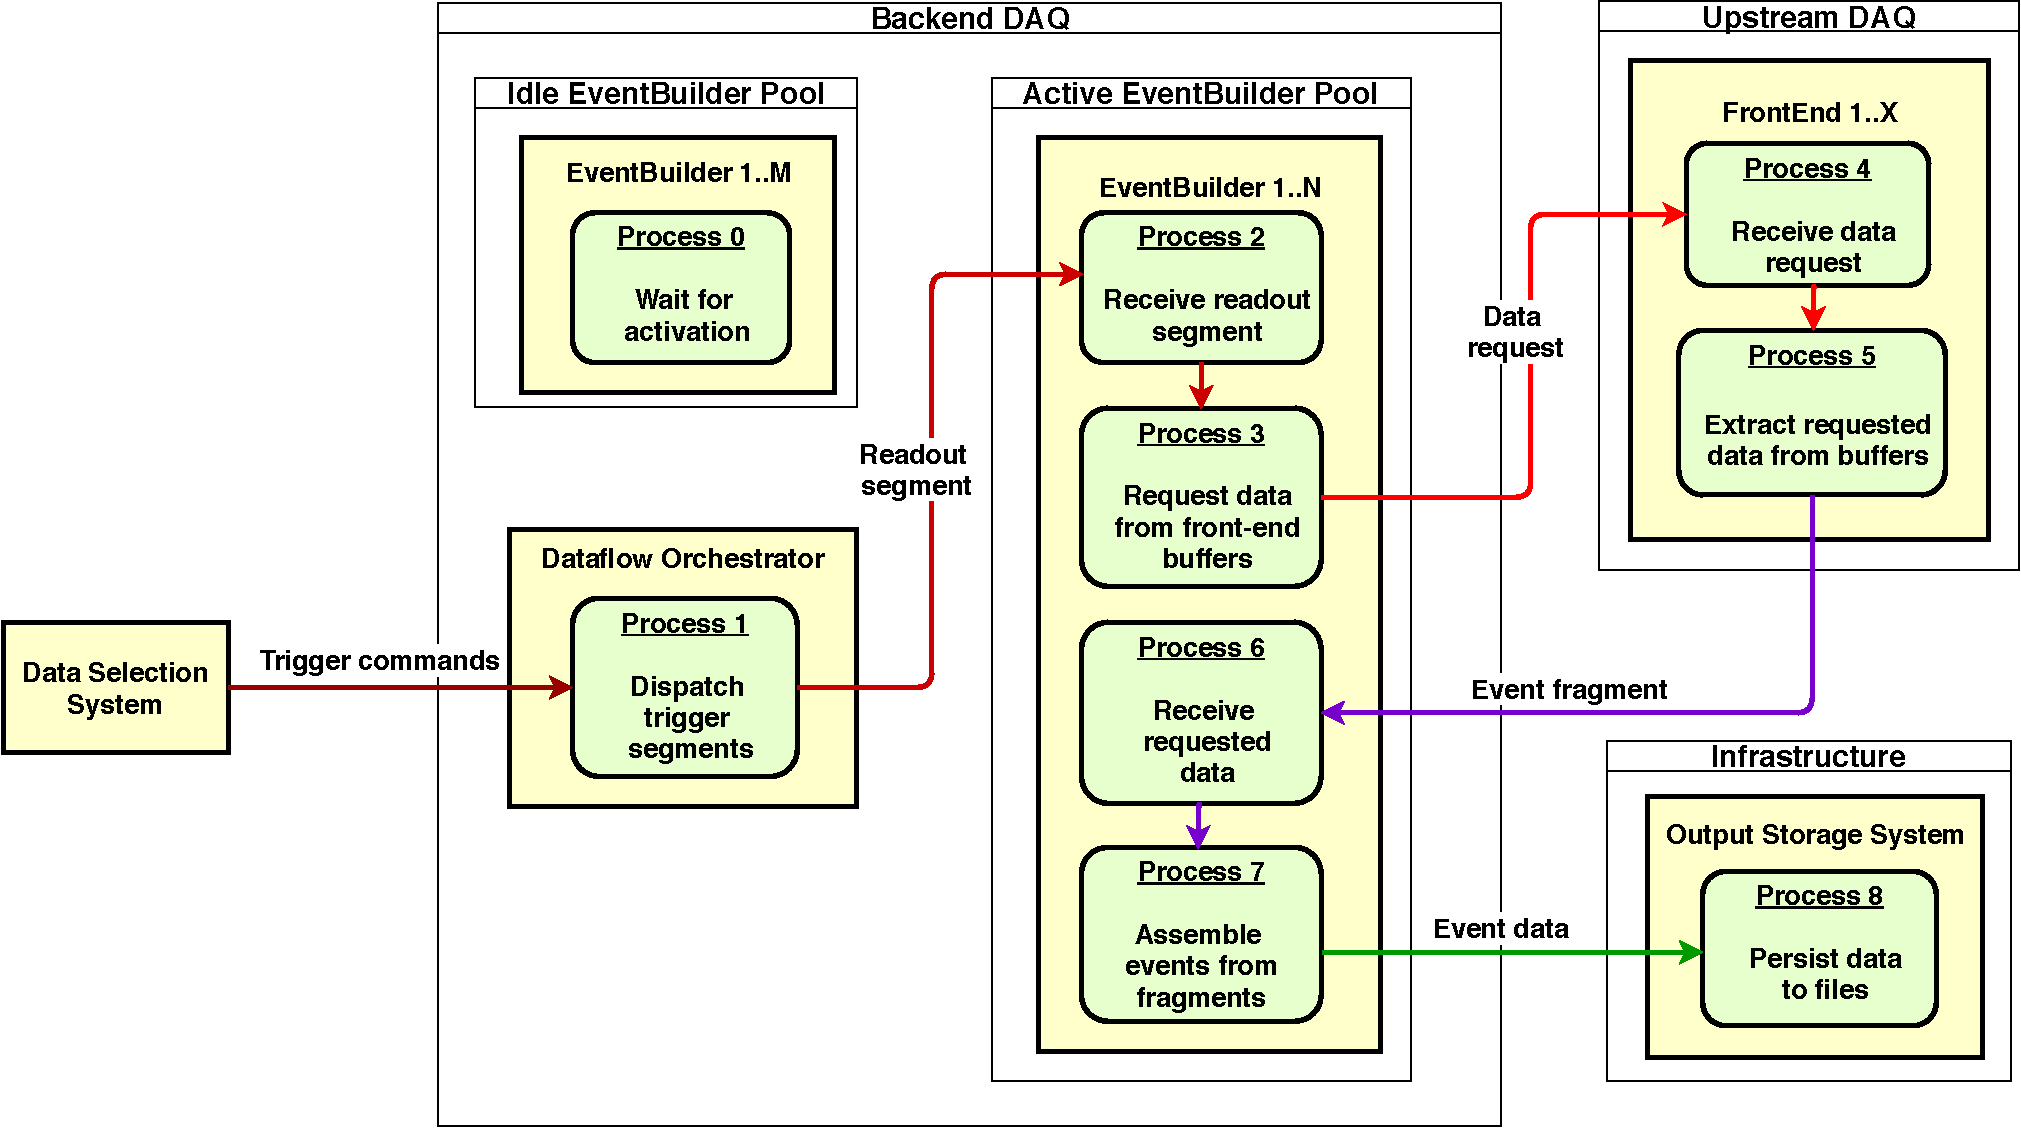
\includegraphics[width=0.8\textwidth]{daq-backend.pdf}
\end{dunefigure}

\begin{itemize}
\item \dword{daqdfo} accepts a time ordered stream of \dwords{trigcommand} and dispatches each for execution possibly by first splitting up each command into one or more contiguous segments.
\item Each segment will then be dispatched to an \dword{eb} process as described in Section~\ref{sec:fd-daq:design-event-builder} for execution.
\item Execution entails interpreting the trigger command segment and querying the appropriate \dword{fe} buffer interfaces to request data from the period of time. 
\item Requests and their replies may be sent synchronously, and replies are expected even if data has already been purged from the \dword{fe} buffer.
\item The data received may then undergo processing and aggregation until finally it is saved to one or more files on the output storage system before custody is transferred offline.
\end{itemize}
%\fixme{Add time order requirement on DS above}
%\fixme{Add return-empty-response requirement to buffer above}



\subsubsection{Event builder}
\label{sec:fd-daq:design-event-builder}
%\fixme{module-generic}
%\metainfo{Explain art\dword{daq}, handling of trigger commands by asynchronous, parallel queries to front end Data Selector (but take care not to duplicate between here and in the overview).}

The \dword{daq} back-end subsystem will provide the instances of the \dfirst{eb}.
As described above, each will request selected data from the appropriate \dfirst{daqfbi} as addressed by a consumed trigger command segment. 
An \dword{eb} will aggregate the selected data and potentially apply processing and reduction (Section~\ref{sec:fd-daq:design-data-reduction}) as well as monitor its quality while in flight.
Finally it will record the resulting data to the output storage system.
The final output files shall use data schema and file formats as described in Section~\ref{sec:fd-daq:design-data-model}.



\subsubsection{Data Quality Monitoring}
\label{sec:fd-daq:design-data-quality}

Section~\ref{sec:daq:design:ccm:monitoring} described a monitoring system for the \dword{daqccm} subsystems. 
Monitoring the quality of the information held in the detector data itself is critical to promptly responding to unexpected conditions and maximizing the quality of acquired data. 
A \dword{daq} \dfirst{dqm} system will be developed to provide functionality for the infrastructure, visualization and algorithms required to continuously process a subset of the detector data so that prompt summaries may be provided for human consumption.
This system will be designed to allow it to evolve as the detector and its data is understood during commissioning and early operation and to cope with any evolution of detector conditions.
Many software modules will be developed offline, so the \dword{dqm} subsystem will facilitate their reuse when applied to samples of detector data.


\subsubsection{Data Model}
\label{sec:fd-daq:design-data-model}
\fixme{module-generic}

\metainfo{Describe the data model. 
  This isn't a strict schema just things like how various parts of the
  detector readout map to files, etc.}

\subsubsection{Output Buffer}

\metainfo{Describe the output buffer system, how it's shared with offline, data hand-off prototocols.  Responsibility scope (eg, who handles transfer to FNAL).}

The output buffer system is a hardware resource provided by \dword{daq} and used offline by \dword{dune}. 
It has two primary purposes. 
First, it decouples producing content in operating \dword{daq} from transferring that content from the far site to archive storage units and offline processing. 
Second, it provides local storage sufficient for uninterrupted \dword{daq} operation in the unlikely event that the connection between the \dword{fd} and the Internet is lost. 
Based on very unusual losses of connectivity at major laboratories as well as \dword{fd} sites of other long-baseline neutrino experiments, the output buffer must provide enough storage capacity to retain one week of output given nominal data production. 
The maximum data production rate for the \dword{fd} is set at \SI{30}{\peta\byte/\year}. 
Thus, the output storage buffer must have a capacity of approximately \SI{0.5}{\peta\byte} to service the entire \dword{fd}.
\fixme{How to reference the 30PB/yr requirement?}


\subsection{Timing Distribution and Synchronization System}
\label{sec:sp-daq:design-timing}
%\fixme{single-phase module}
%\fixme{Is it indeed still single-phase specific?}
%\metainfo{Hardware, consumers, links.}

All components of the \dword{fd} use clocks derived from a single \dfirst{gps} disciplined source, and all module components are synchronized to a \SI{62.5}{MHz} clock. 
To make full use of the information from the \dword{pds}, the common clock must be aligned within a single detector %unit 
module with an accuracy of \bigo{\SI{1}{\nano\second}}. 
For a common trigger for a \dword{snb} between modules, the timing must have an accuracy of \bigo{\SI{1}{\milli\second}}.
However, a still tighter constraint is the need to calibrate the common clock to universal time derived from \dword{gps} so the \dword{daqdsn} algorithm can be adjusted inside an accelerator spill, which again requires an absolute accuracy of \bigo{\SI{1}{\micro\second}}.

The \dword{dune} \dword{fd} uses a version of the \dword{protodune} timing
system, where a design principle is to transmit synchronization messages over
a serial data stream with the clock embedded in the data. The format
is described in \citedocdb{1651}. The timing system design is
described in detail in \citedocdb{11233}.

Central to the timing system are four types of signals:
\begin{itemize}
\item a \SI{10}{\mega\hertz} reference used to discipline a stable master clock,
\item a \dfirst{pps} from the GPS,
\item a \dword{ntp} signal providing an absolute time for each \dword{pps}, and
\item an \dfirst{irig} time code signal
  used to set the timing system 64-bit time stamp.
\end{itemize}
%The timing system associates the \dword{gps} time to its master clock by using the latter to stamp the arrival time of the \dword{pps} of the former. To provide an absolute time to the nearest second the information from \dword{ntp} is used.
%\fixme{This may no longer be correct.  Will NTP be used and the host computer clock consulted for the absolute time?  Will PTP used in its stead?  How does IRIG fit in?  Finally, this sentence, however it needs to be written, is redundant with the itemized list.}

The timing system synchronization codes are distributed to the \dword{daq} readout components in the \dfirst{cuc} and the readout components on the cryostat via single mode fibers and passive splitters/combiners.
All custom electronic components of the timing system are contained in two \dword{utca} shelves; at any time, one is active while the other serves as a hot spare.
The \SI{10}{MHz} reference clock and the \dword{pps} signal are received through a single-width advanced mezzanine card (\dword{amc}) at the center of the \dword{utca} shelf.
This master timing \dword{amc} is a custom board and produces the timing system signals, encoding them onto a serial data stream.
This serial data stream is distributed over a backplane to a number of fanout \dwords{amc}.
The fanout \dword{amc} is an off-the-self board with two custom \dwords{fmc}.
Each \dword{fmc} has four \dword{sfp} cages where fibers connect the timing system to each detector component (e.g., \dword{apa}) or where direct attach cables connect to other systems in the \dword{cuc}.

To provide redundancy, two independent GPS systems are used,
one with an antenna at the surface of the Ross shaft, and the other
with an antenna at the surface of the Yates shaft. Signals from either
GPS are fed through optical single mode fibers to the \dword{cuc}, where
either GPS signal can act as a hot spare while the other is active. 
Differential delays between these two paths are resolved by a second pair of fibers, one running back from the timing system to each antenna.

\subsection{Design Validation and Development Plan}
\label{sec:sp-daq:design-validation}
\fixme{single-phase module}

The \dword{dune} \dword{fd} \dword{daq} design will be validated and developed using the following strategy:
\begin{itemize}
\item Use \dword{protodune} as a design demonstration platform. 
\item Use vertical slice teststands for further development and testing of
  individual \dword{daq} subsystems and for key aspects of the
  overall \dword{daq}
\item Use horizontal slice tests to demonstrate scaling the design where the multiplicity of components in layers is important.
\item Use \dword{fd} MonteCarlo simulations and studies to augment
  demonstrations using \dword{protodune} and the testing at vertical slice teststands.
\item Cross-check against developments and measurements from other ongoing
  LArTPC experiments.
\end{itemize}

This strategy reflects the current \dword{daq} project schedule, which
comprises several phases, including an intense development phase
running through 2020 that culminates in an engineering design
review (EDR) in Q4 of 2020. At this milestone, the system design will be
finalized and shown to be capable of meeting the requirements of the
final \dword{daq} system. After the development phase, a
pre-production phase begins and will end with a production readiness
review (PRR). By then, final designs of all components
will be complete.

The following subsections summarize past, ongoing, and planned
development and validation studies and identifies how anticipated outcomes
will be used to finalize the \dword{daq} design.
%  Put each validation study (performed or future) in a subsubsection
 % and describe either \textbf{how it justifies a decision} or
 % \textbf{how its outcome will be used to make a decision in the
  %  future}.}

\subsubsection{Ongoing  \dword{felix}  Throughput Demonstration at \dword{protodune}}
\label{sec:sp-daq:validation-pdune-felix}
%\fixme{single-phase module}

%\metainfo{Describe how the  \dword{felix}  \dword{daq} at \dword{protodune} demonstrates a
 %  \dword{felix} +CPU approach. 
 % Describe the elements that are same or similar (full-rate to host
 % RAM buffer) and different (higher-rate but external trigger).}

The  \dword{felix}  \dword{daq} at \dword{protodune} partly demonstrates the front-end readout scheme for
the PDS system, as well as the  \dword{felix} +CPU readout approach for the
TPC. The elements of the \dword{protodune}  \dword{felix}  \dword{daq}, which are the
same in \dword{dune}, have already demonstrated the
reception of raw data at full rate from a single \dword{apa} to a 
 \dword{felix}  card and  \dword{felix}  host RAM buffer; upon receiving an external trigger, the
data is propagated to the back-end system. The back-end system
operates similarly to \dword{dune} itself. What differs in the final \dword{dune}
implementation is that neither in the host CPU or
GPU, nor in the added \dword{fpga} functionality does data processing  trigger primitive  generation and subsequent processing
of \dwords{trigprimitive} through the \dword{daqdsn} system. Another
significant difference is the much higher rate of data propagation from the
host RAM to the back-end system in \dword{protodune} than anticipated for the \dword{fd}. Future development
will concentrate on data processing and \dword{daqdsn}.  This is described in more detail in Section~\ref{sec:sp-daq:validation-pd-demonstrator}.

\subsubsection{Ongoing RCE Throughput Demonstration at \dword{protodune}}
\label{sec:sp-daq:validation-pdune-rce}
%\fixme{single-phase module}

The RCE \dword{daq} in \dword{protodune} demonstrates part of the readout scheme for
the  \dword{felix} +FPGA readout approach for the TPC. In particular, it
shows that real-time TPC data processing for lossy
and lossless compression can be facilitated in FPGA, achieving
compression factors consistent with those expected based on observed
\dword{protodune} noise levels. In the future, the system will be used
to demonstrate how \dwords{trigprimitive} are generated in FPGA as
described in Section~\ref{sec:sp-daq:validation-pd-demonstrator}.

\subsubsection{Validation of Trigger Primitives in Software}
\label{sec:sp-daq:validation-software-trigger-primitives}
%\fixme{single-phase module}

Generating \dwords{trigprimitive} in CPU or GPU software has not
yet been demonstrated \textit{in situ} in \dword{protodune}, but it has been
demonstrated in simulations, using real data from \dword{protodune}, on a
server with specs similar to those 
of the  \dword{felix}  host server at \dword{protodune}.

The algorithm is described in detail in \cite{docid-11236}; a Monte Carlo test has demonstrated the algorithm can do real-time processing of one APAs worth
of collection wire data. This test was performed on a Xeon Gold 6140
system, where four (4) threads (cores) were sufficient to keep
up with the detector data rate. The algorithm begins with pedestal removal by
finding the mean of any given wire waveform baseline using a frugal
streaming approach. A look-ahead approach was used to stop
updating the pedestal when it became clear that a potential signal
had been found. Noise filtering in the form of a 7-tap low-pass FIR
filter will be applied as an intermediate step
between pedestal subtraction and hit finding. The hit finding
algorithm is a simple threshold-discriminator. Using Monte Carlo, a hit
threshold of 10 \dword{adc} counts, corresponding to 1\/4 MIP for deposits originating at the cathode, yields hit primitives dominated by
$^{39}$Ar and maintains 100\% efficiency to MIP hits. This is robust against noise level 
increases of 50\% above the default \dword{dune} Monte Carlo settings \cite{docid-11275}. 

Tests of \dword{trigprimitive} generation on very early \dword{protodune} data have also been
performed. Because of its surface
location and the known noisy channels included in this study,
\dword{protodune} \dword{trigprimitive} generation rates level off to a floor rate higher than a threshold
of approximately 16 \dword{adc} counts. Although the total rates are much higher than
anticipated for DUNE, the algorithm performance is promising and should improve as \dword{protodune} continues
to run and improve its noise understanding.

\subsubsection{Validation of Trigger Primitives in Firmware}
\label{sec:sp-daq:validation-firmware-trigger-primitives}
%\fixme{single-phase module}

While \dword{trigprimitive} generation in firmware has not yet been
demonstrated in the RCE system in \dword{protodune}, candidate
algorithms are being developed and will be deployed in an \dword{fpga}
for both \dword{protodune} and other demonstrators. 

On the other hand, \microboone has been able to
successfully implement dynamic baseline estimates and subtraction
for region-of-interest hit finding in an \dword{fpga} \cite{NNN18}.
%\metainfo{Succinctly describe algorithm, include physics and computing
%  performance numbers.}

\subsubsection{Validation of Hierarchical Trigger Layers}

As described in Section~\ref{sec:sp-daq:design-selection-algs}, the \dfirst{daqdss} is structured as a layered hierarchy. 
It must take in constant, high-rate data and output a minuscule rate that provides summary of activity in the data (trigger commands).
To do this, it is structured in layers (primitive, candidate, command) and each layer requires certain multiplicity that spans multiple host computers communicating over the local high-speed but commodity network. 
The algorithms, host computer multiplicity, the \dfirst{ipc} system and its network traffic must be demonstrated at scale.
This will require development of the following elements:

\begin{itemize}
\item A model of \dword{trigprimitive} rates and will be developed that is parameterized by signal, background and noise.  This model will be informed by \dword{protodune} and simulation studies.  The model will include the data density per unit of front-end computing as informed by the \dword{trigprimitive} validation work described above.
\item Likewise an initial model of trigger candidate rates will be developed and concurrently prototype trigger candidate algorithms will be developed and applied to \dwords{trigprimitive} produced by their validation work (again, described above).
\item Trigger candidate message schema and IPC application-level protocol (described more below) for their transfer will be developed.
\item Validation will involve implementing these models, prototype algorithms, schema, etc,  initially at a small-scale on a single high-core computer and using throttled localhost connectivity.
\item The full-scope system will require \bigo{100} host computers, but contiguous branches of the hierarchy can and will be fully tested with \bigo{20} host computers. 
  These hosts will support 10 Gbps networking (actual or throttled) to match the expected networking. 
  In some cases higher bandwidth connectivity may be investigated if bottlenecks are discovered. 
\end{itemize}



\subsubsection{Validation of High Level Trigger in Software}


\subsubsection{Prototype Inter-process Communication System}
\label{sec:fd-daq:validation-demonstrators}
\fixme{module-generic}

A prototype \dfirst{ipc} system is currently under development. 
Some of the goals of this prototype are:

\begin{itemize}
\item Evaluate raw data throughput, particularly via inter-thread communication transport.
\item Evaluate packet rate limitations, particularly those relevant to the hierarchical trigger layers of the \dword{daqdsn} system described in Section~\ref{sec:sp-daq:design-selection-algs}.
\item Understand the required message schema and protocols.
\item Prototype high-level functionality described in Section~\ref{sec:daq:design-ipc} such as zero-downtime reconfiguration, self healing and the patterns required \dword{daqccm} as described in Section~\ref{sec:fd-daq:design-run-control}.
\item Investigate scaling in terms of performance and software complexity management.
\item Provide functional support for the vertical and horizontal slice tests described above.
\end{itemize}

The prototype software development follows some design principles:

\begin{itemize}
\item The \dword{daq} is modeled as a cyclic, data flow graph.
\item Graph nodes in the graph perform transformations and may consume data input from and produce data output to other nodes.
\item Graph edges connect nodes through ports associated with a network socket.
\item Graph construction emerges by initiating connections locally.
\item Executable processes provide one or more nodes that operate asynchronously from one-another governed only by the flow of messages across their shared edges.
\item Construction of nodes in executable processes and larger graph construction is dynamic governed by initial user configuration and later by messages flowing in the graph itself.
\end{itemize}

The prototype development is based on the well-established, high-quality free software from the ZeroMQ group.
Some of the reasons for selecting their technology include:
\begin{itemize}
\item ZeroMQ software follows a well layered set of software libraries that emphasize portability, high performance, fault tolerance, minimal software dependency and long-lived use and support.
\item A wide variety of language bindings exist, importantly C/C++ for high performance and Python for fast development are two of the best supported.
\item ZeroMQ abstracts functionality in important ways such as concrete implementation of high level communication patterns (eg, pub/sub) and high-level independence from low-level transport mechanism (three are supported: inter-thread queues, inter-process Unix-domain sockets and inter-computer network sockets). 
\item It supports a truly decentralized system design (this is the ``Zero'' in ``ZeroMQ'') critical to satisfying the requirements on robustness.  In particular the ZeroMQ project Zyre provides a distributed, low-latency \dword{daqdispre} system.
\item ZeroMQ has been evaluated favorably CERN~\cite{Dworak:2012mf} and has been used in various \dword{daq} contexts in other experiments.
\end{itemize}

Initial prototype tests have demonstrated that the raw data throughput of ZeroMQ inter-thread transport is sufficient for use in even the highest rate \dword{daq} context (input to \dword{trigprimitive} production).
Rate tests of small packets have been performed to gauge ZeroMQ ability to handle high packet rate \dword{trigprimitive} or trigger candidate data. 
These tests have so far been performed merely on Gbps networks. 
Given reasonably linear scaling as well as benchmarks preformed on faster networks by others, ZeroMQ will perform adequately for DUNE FD \dword{daq} purposes.

The ZeroMQ-based prototype software will continue to be developed with the goal to understand how to manage software and configuration complexity and to participate in the other demonstrators described in this section. 


\subsubsection{Planned \dword{protodune} \dword{daq} Demonstrator}
\label{sec:sp-daq:validation-pd-demonstrator}

A demonstration of the \dword{daq} system design based in \dword{protodune} is
planned for 2020. The key components are the front-end readout, timing
system, and \dword{daqdsn} systems. A full vertical slice through the
timing and readout system will be constructed, with
TPC and PDS detectors, as well as calibration systems. Although a full-scale
demonstration of the \dword{daqdsn} system cannot be achieved with
\dword{protodune}, the basic infrastructure will be demonstrated and
used to self-trigger \dword{protodune}.

The high-level goals will be to demonstrate and validate
integration of \dword{fe} with TPC and PDS electronics, 
data throughput for a single \dword{fe} instance 
readout data processing for a single \dword{fe} instance 
\dword{trigprimitive} generation for a single front-end instance 
distribution of timing and control signals to detector \dwords{fe} 
data selection infrastructure and self-triggering  and 
integration with calibration systems.

The components used in the \dword{protodune}
demonstrator will be assembled in 2019, and their operation will
be verified in standalone tests. For \dword{fpga} processing, the
initial version of firmware will be demonstrated in \dword{fpga} development
cards, and an integration test will be conducted in 2019 with a
prototype \dword{fpga} processing module and the  \dword{felix} \dword{fe}.


\subsubsection{Planned Vertical Slice Teststands}
\label{sec:sp-daq:validation-demonstrators}
%\fixme{single-phase module}
%\metainfo{Describe VST demonstrators and why we must build them.}

A number of vertical slice teststands will be built to allow
development and testing of individual parts of the \dword{daq} system
as well as testing of key aspects of the design and overall scalability. At minimum, the following teststands
will be constructed:
\begin{itemize}
\item \Dword{daqdsn}: List aims. One option is to construct a
  full-scale \dword{daqdsn} system using fake data 
sources, which could be simulated or real (pre-recorded)
\dword{protodune} data,
or both, subject to available resources. Another option is to identify
likely failure points and/or bottlenecks and perform
small-scale tests that stress the critical parts of the corresponding
infrastructrure. The criteria for those tests will be defined beforehand.
\item Back-end system: List aims. (Not finished)
\end{itemize}

Other than these dedicated vertical slice teststands, a number of
\dword{daq} development kits will be available for other detector and
calibration consortia to support 
their own development, production, and quality assurance programs. The \dword{daq} 
kit will also form the basis for testing at the ITF beginning in 2022. This will
also allow validating the detector and \dword{daq} interfaces. %A
%single \dword{daq} kit will be capable of handling data from a single APA. 

\section{Production, Assembly, Installation and Integration}
\label{sec:sp-daq:production}

(Not finished.)

\metainfo{Describe how hardware, firmware and software will produced. }

\metainfo{Describe how we get stuff in place underground (and in the
  ITF), how we will put it all together and make sure it works. 
  What can we do to minimize the effort needed underground both in
  terms of physical work but also in working out the bugs both in
  individual processes and in emergent behavior of the system as a
  whole?}

\subsection{Computing Hardware}

\subsection{Custom Hardware Fabrication}

\subsection{Software and Firmware Development}
\metainfo{Processes and practices.}

\subsection{ITF}

\section{Cost, Schedule, Safety and Risk Summary}
\label{sec:sp-daq:cost}
\metainfo{
Include cost summary and table here.
Include schedule summary and table here.
Include risk summary and table here.}

\begin{dunetable}
[Data Acquisition System Cost Summary]
{p{0.7\textwidth}p{0.2\textwidth}}
{tab:sp-daq:costsumm}
{Data Acquisition System Cost Summary (made-up numbers)}
 Item & Core Cost (k\$ US) \\ \toprowrule
 (item 1) & \num{67.0} \\ \colhline
 (item 2) & \num{57.8} \\ \colhline
 ... & ... \\ \colhline
 (last item)& \num{47.4} \\
\end{dunetable}

\begin{dunetable}
[Data Acquisition System Schedule]
{p{0.65\textwidth}p{0.25\textwidth}}
{tab:sp-daq:sched}
{Data Acquisition System Schedule (made-up dates)}
Milestone & Date (Month YYYY) \\ \toprowrule
(item 1) & October 2020 \\ \colhline
(item 2) & March 2021 \\ \colhline
... & ... \\ \colhline
(last item)& June 2023 \\
\end{dunetable}


\begin{dunetable}
[Data Acquisition System Risk Summary]
{p{0.15\textwidth}p{0.75\textwidth}}
{tab:sp-daq:risks}
{Data Acquisition System Risk Summary}
ID & Risk \\ \toprowrule
(id 1) & risk text \\ \colhline
(id 2) & risk text \\ \colhline
... & ... \\ \colhline
(last id)& risk text \\
\end{dunetable}
